\documentclass[11pt]{cauchy}

\usepackage{mlmodern}
\usepackage{mathsphystools}
\usepackage{thmstyles}
\usepackage{graphicx}
\graphicspath{{images/}}

\usepackage{tikz}
\usepackage{tikz-cd}
\tikzset{>=stealth}
\tikzcdset{arrow style=tikz}

\setlist[enumerate,1]{label=(\roman*)}
\setlist[enumerate,2]{label=\alph*.}

\newcommand{\oB}{B}
\newcommand{\cB}{\overline{B}}
\newcommand{\cover}[1]{\mathcal{#1}}

\title{Norms, Metrics and Topologies}
\subtitle{Lecture Notes}
\author{Rashid M. Talha}
\affiliation{School of Natural Sciences, NUST}
\date{\today}
\begin{document}

%!TEX root = ../main.tex
\setcounter{page}{0}
\thispagestyle{fancy-blank}
\begingroup
% \vphantom{Optional note}
% {\large Optional note\par}
\vspace*{35mm}
{\huge\bfseries\utitle\par}

\vspace*{5mm}
{\Large\usubtitle\par}

\vspace*{4mm}
{\rule{\linewidth}{0.5mm}\par}
\vspace*{4mm}

{\large\bfseries\uauthor\par}\vspace*{1mm}

{\large\itshape\uaffiliation\newline}
{\large\itshape\udate\newline}
{\large\itshape{Email: rmathsphys@gmail.com}\par}

\vfill
% {\large Optional note\par}
\endgroup
\clearpage


\frontmatter
\tableofcontents\clearpage

%!TEX root = ../main.tex

\clearpage
\phantomsection
\addcontentsline{toc}{section}{Abstract}
\begin{adjustwidth}{0.1\textwidth}{0.1\textwidth}
\begingroup
\null\vspace{0.2\textheight}
\begin{center}
{\bfseries\Large Abstract}\par\vspace{2em}

Lorem ipsum dolor sit amet, consectetur adipisicing elit, sed do eiusmod tempor incididunt ut labore et dolore magna aliqua. Ut enim ad minim veniam, quis nostrud exercitation ullamco laboris nisi ut aliquip ex ea commodo consequat.
\end{center}
\endgroup
\end{adjustwidth}
\clearpage
% %!TEX root = ../main.tex

\clearpage
\phantomsection
\addcontentsline{toc}{section}{Acknowledgements}
\begin{adjustwidth}{0.1\textwidth}{0.1\textwidth}
\begingroup
\null\vspace{0.2\textheight}
\begin{center}
{\bfseries\Large Acknowledgements}\par\vspace{2em}

Lorem ipsum dolor sit amet, consectetur adipisicing elit, sed do eiusmod tempor incididunt ut labore et dolore magna aliqua. Ut enim ad minim veniam, quis nostrud exercitation ullamco laboris nisi ut aliquip ex ea commodo consequat.
\end{center}
\endgroup
\end{adjustwidth}
\clearpage

\mainmatter
%!TEX root = ../main.tex
\section{Preliminary Topics}
\subsection{Sets}
BASICS OF SETS. SOME NOTATION.

\subsection{Functions}
BASICS OF FUNCTIONS. THE INVERSE-IMAGE (PRE-IMAGE). THE EXISTENCE AND UNIQUENESS OF THE INVERSE. SOME NOTATION.

\subsection{Inequalities}
BASICS OF INEQUALITIES.
%!TEX root = ../main.tex
\section{Normed Vector Spaces}
\begin{ndfn}[Norm]
  Let $V$ be a vector space over $\R$. A norm on $V$ is a function $\norm{\cdot}:V\to\R$ with the following properties
  \begin{enumerate}
  \item $\norm{v} = 0 \iff v =0$, for $v \in V$, \hfill (definiteness)
  \item $\norm{\lambda v} = \abs{\lambda}\norm{v}$, $\forall \lambda \in \R$ and $\forall v \in V$, \hfill (absolute homogeneity)
  \item $\norm{u+v} \leq \norm{u} + \norm{v}$, $\forall u,v \in V$. \hfill (triangle inequality)
  \end{enumerate}
\end{ndfn}

\begin{ndfn}[Normed space]
  Let $V$ be a vector space, and let $\norm{\cdot}$ be a norm on $V$. The pair $(V, \norm{\cdot})$ is called a normed (vector) space.
\end{ndfn}

Some authors give a slightly different, but equivalent definition of the norm.

It should be clear from the definition that the vector space structure on $V$ is a necessity, since the axioms of being a norm rely on the existence of $0 \in V$ (the additive identity), scalar multiplication, and addition. We shall focus on the case where the underlying field is the real numbers, $\R$, however, an analogous theory can be developed in the case of other fields, for example, the complex numbers $\C$.

The idea behind defining a norm $\norm{\cdot}$ is that $\norm{x}$ should give us a measure of the \emph{magnitude} of the vector $x$. And magnitudes (or lengths) should be non-negative. So, the norms should be non-negative valued. The next result confirms this property. Some authors directly require $\norm{\cdot}:V\to[0,\infty)$, which simply gives the following proposition the status of an axiom.

\begin{nprop}[Non-negative valued]
  Let $\norm{\cdot}:V\to\R$ be a norm on $V$. Then, $\forall x \in V, \norm{x} \geq 0$.
\end{nprop}
\begin{proof}
  Observe the following
  \begin{equation*}
    0
    \overset{\text{(i)}}{=} \norm{0}
    = \norm{x+(-x)}
    \overset{\text{(iii)}}{\leq} \norm{x} + \norm{-x}
    \overset{\text{(ii)}}{=} \norm{x} + \abs{-1}\norm{x}
    = \norm{x} + \norm{x}
    = 2\norm{x}.
  \end{equation*}
  So, $2\norm{x} \geq 0$ for all $x \in V$, from which we conclude that $\norm{x} \geq 0, \forall x \in V$.
\end{proof}

Note that this proof works even when $V$ is a vector space over a general field $K$.

\begin{nprop}[Normed subspace]
  Let $(X, \norm{\cdot})$ be a normed space, and let $Y$ be a vector subspace of $X$. Then, $(Y, \norm{\cdot})$ is also a normed space, using the same norm as $X$. $(Y, \norm{\cdot})$ is called the normed subspace of $(X, \norm{\cdot})$. More precisely, this proposition claims that the function $N:Y \to \R$ with $N(y) \coloneq \norm{y}$, for all $y \in Y$, is a norm.
\end{nprop}
\begin{proof}
  Exercise.
\end{proof}

\begin{nex}
  Let $\norm{\cdot}_a$ and $\norm{\cdot}_b$ be any two norms on $V$. Do the following satisfy the definition of a norm
  \begin{enumerate}
  \item $\norm{\cdot}_a$ + $\norm{\cdot}_b$
  \item $\lambda\norm{\cdot}_a + \mu\norm{\cdot}_b$, for $\lambda, \mu \in \R$.
  \item $\norm{\cdot}_a \times \norm{\cdot}_b$
  \item $\sqrt{\norm{\cdot}_{a}}$
  \item $\norm{\left(\norm{\cdot}_b\right)}_{a}$, with the appropriate changes in domain.
  \end{enumerate}
\end{nex}

Let $V$ be a finite dimensional vector space over $\R$. Then, a result from introductory linear algebra shows that $V \cong \R^n$. Define the family of functions $\norm{\cdot}_{p}:\R^n \to \R$,
\begin{equation*}
  \norm{x}_{p} \coloneq \left(\sum_{j=1}^{n} \abs{x_j}^{p}\right)^{1/p}
  \quad\text{and}\quad
  \norm{x}_{\infty} \coloneq \max \set{x_1, \dots, x_n},
\end{equation*}
for $p \in [1,\infty)$ and $x = (x_1, \dots, x_n) \in \R^n$. Despite the suggestive notation, we have not yet claimed that these functions are valid norms.

\begin{nex}
  Show that the functions $\norm{\cdot}_{1}$ and $\norm{\cdot}_{\infty}$, are norms on $\R^n$.
\end{nex}

\begin{nex}
  Show that the function $\norm{\cdot}_{p}$, for $p \in (1,\infty)$, satisfies property (i) and (ii) of being a norm.
\end{nex}

\begin{remark}
  Indeed it will be shown later that $\norm{\cdot}_{p}$ is a norm on $\R^n$, but it will be extremely difficult to show directly that it also satisfy the triangle inequality. In order to establish the triangle inequality we will have to develop an alternative method.
\end{remark}

\begin{ndfn}
  Let $(V, \norm{\cdot})$ be a normed space. We define
  \begin{enumerate}
  \item the open unit ball: $\oB_{V} \coloneq \set{v \in V \st \norm{v} < 1}$
  \item the closed unit ball: $\cB_{V} \coloneq \set{v \in V \st \norm{v} \leq 1}$
  \end{enumerate}
\end{ndfn}
These sets depend on the norm that is being used on $V$.

The closed unit balls produced by the $\ell_{1}$, $\ell_{2}$, and $\ell_{\infty}$ norms on $\R^2$ are shown below.
\begin{center}
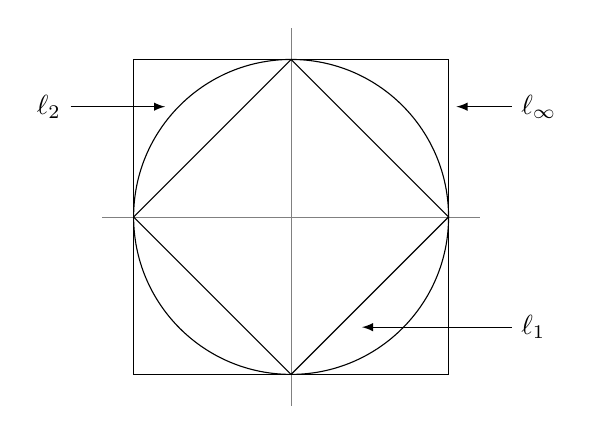
\begin{tikzpicture}[scale=2]
  \draw[help lines] (-1.2,0) -- (1.2,0);
  \draw[help lines] (0,-1.2) -- (0,1.2);
  \draw circle (1cm);
  \draw (1,0) -- (0,1) -- (-1,0) -- (0,-1) -- cycle;
  \draw (1,1) -- (-1,1) -- (-1,-1) -- (1,-1) -- cycle;

  \draw[-latex] (1.4, 0.7) node[anchor=west] {$\ell_{\infty}$} -- +(-0.35, 0);
  \draw[-latex] (-1.4, 0.7) node[anchor=east] {$\ell_{2}$} -- +(0.6, 0);
  \draw[-latex] (1.4, -0.7) node[anchor=west] {$\ell_{1}$} -- +(-0.95, 0);
\end{tikzpicture}
\end{center}

\begin{ndfn}[Convex sets]
  Let $V$ be a vector space. A set $X \subseteq V$ is called convex if $\forall x,y \in X$, and $\forall \lambda \in (0,1)$
  \begin{equation*}
    (1-\lambda) x + \lambda y \in X.
  \end{equation*}
\end{ndfn}
Geometrically, this is saying that $X$ is convex if the line segment joining any every pair of points in $X$, lies entirely within $X$.

\begin{ndfn}[Convex functions]
  A function $f : A \subseteq \R \to \R$ is called convex if $\forall x,y \in A$, and $\forall \lambda \in (0,1)$
  \begin{equation*}
    f\left((1-\lambda) x + \lambda y\right) \leq (1-\lambda) f(x) + \lambda f(y).
  \end{equation*}
\end{ndfn}
Therefore, a function is convex exactly when its graph lies beneath (or along) the line segment joining any two points on the graph. Common examples of convex functions are $x^2$ and $e^x$ on $\R$.

\begin{nprop}
  Let $(V, \norm{\cdot})$ be a normed space. The sets $\oB_{V}$ and $\cB_{V}$ are convex.
\end{nprop}
\begin{proof}
  We shall prove this for $\cB_{V}$. Take $a, b \in \cB_{V}$, and $\lambda \in (0,1)$. Then,
  \begin{equation*}
    \norm{(1-\lambda) a + \lambda b}
    \leq (1-\lambda) \norm{a} + \lambda \norm{b}
    \leq (1-\lambda) + \lambda
     = 1.
  \end{equation*}
  Therefore, $(1-\lambda) a + \lambda b \in \cB_{V}$. So, $\cB_{V}$ is convex.

  The proof for the convexity of $\oB_{V}$ is analogous.
\end{proof}

\begin{nprop}
\label{thm:convexity}
  Suppose $f \in C^2 ((a,b))$ and $f \in C^1 ([a,b])$. If $f''(x) \geq 0$, for all $x \in [a,b]$, then $f$ is convex on $[a,b]$.
\end{nprop}
\begin{proof}
  The proof is left as an exercise to the reader.
\end{proof}

\begin{nlemma}
  The function $f : \R \to [0,\infty)$ with $x \mapsto \abs{x}$ is convex.
\end{nlemma}
\begin{proof}
  To be completed. Uses the MVT.
\end{proof}

\begin{nlemma}
  The function $f : [0,\infty) \to \R$ with $x \mapsto x^p$ is convex, $\forall p \in [1,\infty)$.
\end{nlemma}
\begin{proof}
  The given function is a polynomial, so it is infinitely differentiable, with
  \begin{equation*}
    f''(x) = p(p-1)x^{p-2}.
  \end{equation*}
  Now,
  \begin{equation*}
    p \in [1,\infty), x \in [0,\infty) \implies p, (p-1), x, x^{p-2} \geq 0.
  \end{equation*}
  Therefore, $f''(x) \geq 0$, for all $x$ in the given domain.

  Proposition (\ref{thm:convexity}) then states that $f(x) = x^p$ is convex.
\end{proof}

\begin{nlemma}
  If $f: A \to B$ and $g: B \to C$ are convex functions, then $g \circ f : A \to C$ is also convex.
\end{nlemma}
\begin{proof}
  Take $x,y \in A$ and $\lambda \in (0,1)$. Then,
  \begin{align*}
  (1-\lambda) (g \circ f)(a) + \lambda (g \circ f)(b)
  &= (1-\lambda) g(f(a)) + \lambda g(f(b))\\
  &\geq g\left((1-\lambda) f(a) + \lambda f(b)\right)\\
  &\geq g\left(f\left((1-\lambda) a + \lambda b\right)\right)\\
  &= (g \circ f)\left((1-\lambda) a + \lambda b\right).
  \end{align*}
  Therefore, $(g \circ f)$ is convex.
\end{proof}

Combining these lemmas, we obtain that $\forall p \in [1,\infty)$, $x \mapsto \abs{x}^{p}$ is a convex function. In other words, $\forall x,y \in \R$, and $\forall \lambda \in (0,1)$,
\begin{equation*}
  \abs{(1-\lambda) x + \lambda y}^{p} \leq (1-\lambda) \abs{x}^{p} + \lambda \abs{y}^{p}.
\end{equation*}

Now, we consider a norm-like function that is required to satisfy all the properties except the triangle inequality. If we require the \emph{closed balls} produced by this function to be convex, then we find that it also ends up satisfying the triangle inequality. So, the next result allows us to establish the triangle inequality by checking the convexity of the induced closed balls.

\begin{nthm}
\label{thm:norm-convex-triangle}
  Let $V$ be a vector space, and consider a function $N : V \to [0,\infty)$ with
  \begin{enumerate}
  \item $N(v) = 0 \iff v =0$, for $v \in V$,
  \item $N(\lambda v) = \abs{\lambda}N(v)$, $\forall \lambda \in \R$ and $\forall v \in V$,
  \item $B \coloneq \set{v \in V \st N(v) \leq 1}$ is convex.
  \end{enumerate}
  Then,
  \begin{equation*}
    N(x+y) \leq N(x) + N(y)
  \end{equation*}
  i.e. $N$ satisfies the triangle inequality, and therefore, $f$ is a norm on $V$.
\end{nthm}
\begin{proof}
  Firstly if $N(x)=0$ then $x=0$, and
  \begin{equation*}
    N(x+y) = N(y) = N(x) + N(y).
  \end{equation*}
  Similarly, for $N(y)=0$, we have $y=0$, so
  \begin{equation*}
    N(x+y) = N(x) = N(x) + N(y).
  \end{equation*}
  Hence, assume $N(x), N(y) \geq 0$, and pick $x, y \in V$. Then, $x/N(x), y/N(y) \in V$ by closure under scalar multiplication. Moreover, $x/N(x), y/N(y) \in B$, since
  \begin{equation*}
    N\left(\frac{x}{N(x)}\right) = \abs*{\frac{1}{N(x)}}N(x) = \frac{N(x)}{N(x)} = 1.
  \end{equation*}
  Similarly for $y/N(y)$.

  By convexity of $B$ we have that
  \begin{align*}
  &\left(1 - \frac{N(y)}{N(x)+N(y)}\right)\frac{x}{N(x)} + \left(\frac{N(y)}{N(x)+N(y)}\right)\frac{y}{N(y)} \in B\\
  &\implies \left(\frac{N(x)}{N(x)+N(y)}\right)\frac{x}{N(x)} + \left(\frac{N(y)}{N(x)+N(y)}\right)\frac{y}{N(y)} \in B\\
  &\implies \frac{x+y}{N(x)+N(y)} \in B\\
  &\implies N\left(\frac{x+y}{N(x)+N(y)}\right) \leq 1\\
  &\implies \frac{N(x+y)}{N(x)+N(y)} \leq 1.
  \end{align*}
  Therefore, $N(x+y) \leq N(x) + N(y)$, as required.
\end{proof}

\begin{ncor}[Minkowski's inequality in $\R^n$]
  For all $p \in [1,\infty)$, if $x, y \in \R^n$
  \begin{equation*}
    \norm{x+y}_{p} \leq \norm{x}_{p} + \norm{y}_{p}.
  \end{equation*}
\end{ncor}
\begin{proof}
  Recall that
  \begin{equation*}
    \norm{x}_{p} \coloneq \left(\sum_{j=1}^{n} \abs{x_j}^{p}\right)^{1/p},
  \end{equation*}
  and consider the closed ball $B = \set{x \in \R^n \st \norm{x}_p \leq 1}$. Then,
  \begin{equation*}
    B = \set{x \in \R^n \st \norm{x}_p \leq 1} = \set{x \in \R^n \st \norm{x}_{p}^{p} \leq 1}.
  \end{equation*}

  We aim to show that $B$ is convex, and then use theorem (\ref{thm:norm-convex-triangle}) to obtain the triangle equality. Note that $\norm{\cdot}_{p}$ already satisfies the properties (i) and (ii) of theorem (\ref{thm:norm-convex-triangle}).

  Now, take any $x,y \in B$ and $\lambda \in (0,1)$. Then,
  \begin{align*}
  \norm{(1-\lambda) x + \lambda y}
  &= \sum_{j=1}^{n} \abs{(1-\lambda) a_j + \lambda b_j^{p}}\\
  &\leq \sum_{j=1}^{n} (1-\lambda) \abs{a_j}^{p} + \lambda \abs{b_j}^{p}\\
  &= (1-\lambda)\sum_{j=1}^{n} \abs{a_j}^{p} + \lambda \sum_{j=1}^{n} \abs{b_j}^{p} \\
  &= (1-\lambda)\norm{a}_{p}^{p}+\lambda\norm{b}_{p}^{p}\\
  &\leq (1-\lambda)+\lambda\\
  &= 1.
  \end{align*}
  Therefore, $\norm{(1-\lambda) x + \lambda y} \leq 1$; i.e. $(1-\lambda) x + \lambda y \in B$. This confirms that $B$ is convex. Theorem (\ref{thm:norm-convex-triangle}) then states that $\norm{\cdot}_{p}$ satisfies the triangle inequality. That is
  \begin{equation*}
  \norm{x+y}_{p} \leq \norm{x}_{p} + \norm{y}_{p}.\qedhere
  \end{equation*}
\end{proof}

\begin{remark}
  This completes the proof that $\norm{\cdot}_{p}$, for $p \in [1,\infty)$, as defined before, fulfils all the requirements of being a norm on $\R^n$.
\end{remark}

Next, we look at equivalent norms and the associated results for their closed (open) unit balls.

\begin{ndfn}
  Let $V$ be a vector space. A norm $\norm{\cdot}_a$ on $V$ is said to be equivalent to another norm $\norm{\cdot}_b$ on $V$ if $\exists c_1, c_2 \in \R$ with $0 < c_1 \leq c_2$, such that
  \begin{equation*}
    c_1 \norm{x}_b \leq \norm{x}_a \leq c_2 \norm{x}_b, \forall x \in V.
  \end{equation*}
  We denote this as $\norm{\cdot}_a \cong \norm{\cdot}_b$.
\end{ndfn}
It is important that the constants $c_1$ and $c_2$ are independent of the element $x \in V$. Clearly, if $\norm{\cdot}_a$ is equivalent to $\norm{\cdot}_b$, then $\norm{\cdot}_b$ is equivalent to $\norm{\cdot}_a$. In fact this is an equivalence relation. (Exercise \& Content for the appendix)

WHAT IS THE POINT OF EQUIVALENT NORMS?

\begin{nprop}
  $\norm{\cdot}_a \cong \norm{\cdot}_b$ if an only if $\exists c_1, c_2 \in \R$ with $0 < c_1 \leq c_2$, such that $c_1 \cB_b \subseteq \cB_a \subseteq c_2 \cB_b$. Here, $\cB_j$ is the closed unit ball generated by the norm $\norm{\cdot}_j$.
\end{nprop}
\begin{proof}
  The proof is left as an exercise to the reader.
\end{proof}

The previous proposition states that if $\norm{\cdot}_a$ is equivalent to $\norm{\cdot}_b$, then the closed unit ball $\cB_a$ is entirely contained within an appropriately scaled version of the closed unit ball $\cB_b$, and that $\cB_a$ also contains an appropriately scaled version of $\cB_b$. Moreover, the converse of this statement is also true.

\begin{nthm}
  All $\norm{\cdot}_p$ norms on $\R^n$ are equivalent.
\end{nthm}

In fact, a more general result holds for the case of $\R^n$: All norms on $\R^n$ are equivalent. As a result, we are free to choose any of these norm to study limits and continuity in $\R^n$, since the results will always be equivalent.

\paragraph{Some other topics of interest.} $\ell^p$ spaces, $L^p$ spaces, other norms on $\R^n$, inner products, norms on $\C^n$.
%!TEX root = ../main.tex
\section{Metric Spaces}
More general than norms is the notion of a metric. The idea is that a metric is a measure of distance between any two elements in a given set; the norm, on the other hand, is a measure of magnitude of each element individually.

COMMENT ABOUT REAL ANALYSIS.

\subsection{Preliminary definitions}
\begin{ndfn}[Metric space]
  Let $X$ be any set. Let $d : X \times X \to \R$ be a function such that
  \begin{enumerate}
  \item $d(x,y) \geq 0, \forall x,y \in X$, \hfill (positive)
  \item $d(x,y) = 0 \iff x=y$, \hfill (definite)
  \item $d(x,y) = d(y,x), \forall x,y \in X$, \hfill (symmetric)
  \item $d(x,z) \leq d(x,y) + d(y,z), \forall x,y,z \in X$. \hfill (triangle inequality)
  \end{enumerate}
  Then, $d$ is called a metric on $X$, and the pair $(X,d)$ is called a metric space.
\end{ndfn}

Unlike a norm, a metric doesn't require the underlying set to be a vector space. While we will often work with sets $X$ that carry a natural vector space structure, the metric properties will be independent from it unless the metric is being \emph{induced} by the norm.

\begin{nprop}[Metric induced by a norm]
  let $(X, \norm{\cdot})$ be a normed vector space. Then $d : X \times X \to \R$ with $d(x,y) \coloneqq \norm{x-y}$ is a metric on $X$. Such a metric is called the metric induced by the norm.
\end{nprop}
\begin{proof}
  Exercise.
\end{proof}

The metric $d:\R^n \times \R^n \to \R$ induced by the Euclidean norm $\norm{\cdot}_2$ is known as the standard (or Euclidean) metric on $\R^n$. When we consider $\R^n$ as a metric space, without specifying the metric, the underlying metric is assumed to be the standard metric.

\begin{negg}
  On $\R^n$ we get a family of metrics induced by the $\norm{\cdot}_p$ norms, for $p\in[1,\infty]$. Explicitly, these are
  \begin{align*}
    d_{p}(\vec{x}, \vec{y}) &= \left(\sum_{i=1}^{n} \abs{x_i - y_i}^{p}\right)^{1/p} \qquad p \in [1,\infty)\\
    d_{\infty}(\vec{x}, \vec{y}) &= \max_{i=1,\dots,n} \set*{\abs{x_i - y_i}} \qquad p = \infty
  \end{align*}
\end{negg}

\begin{negg}[Discrete metric]
  Let $X$ be any set, and consider the function $d_s:X \times X \to \R$ with
  \begin{equation*}
  d_s = \begin{cases}
  0, & x=y\\
  1, & x \neq y
  \end{cases}
  \end{equation*}
  This is a metric in $X$, known as the discrete metric. This is often very useful for producing counterexamples. (Check.)\eggqed
\end{negg}

\begin{negg}[Sunflower metric]
  The function $d:\R^2 \times \R^2 \to \R$ with
  \begin{equation*}
  d = \begin{cases}
  \norm{\vec{x}-\vec{y}}, & \vec{x}\;\text{and}\;\vec{y}\;\text{lie on the same line through}\;(0,0)\\
  \norm{\vec{x}}+\norm{\vec{y}}, & \text{otherwise}
  \end{cases}
  \end{equation*}
  defines a metric on $\R^2$, known as the sunflower metric. (Check.)\eggqed
\end{negg}

\begin{negg}[Jungle river metric]
  Consider the function $d:\R^2 \times \R^2 \to \R$ with
  \begin{equation*}
  d = \begin{cases}
  \abs{y_1 - y_2}, & \text{if}\;x_1 = x_2\\
  \abs{y_1} + \abs{x_1 - x_2} + \abs{y_2}, & \text{otherwise}
  \end{cases}
  \end{equation*}
  This is known as the jungle river metric on $\R^2$. (Check.)\eggqed
\end{negg}

\begin{negg}
  Let $C[a,b]$ denote the set of all real-valued continuous functions on the closed interval $[a,b]$, $f: [a,b] \to \R$. For $p \in [1,\infty)$, the following function defines a metric
  \begin{equation*}
    d_{p}(f,g) = \left(\int_{a}^{b} \abs{f(x) - g(x)}^{p}\d{x}\right)^{1/p}.
  \end{equation*}
  From real analysis we know that a continuous function on $[a,b]$ attains its bounds. So, the following function is well-defined
  \begin{equation*}
    d_{\infty}(f,g) = \max_{a \leq x \leq b} \abs{f(x) - g(x)},
  \end{equation*}
  and satisfies all the conditions for being a metric.\eggqed
\end{negg}

\begin{negg}[Hamming distance]
  A word $w$, of length $n$ is an expression of the form as $w=w_1 w_2 \cdots w_n$, where $w_i$ are symbols (called letters) from a fixed set. The Hamming distance between any two such words $x=x_1 x_2 \cdots x_n$ and $y=y_1 y_2 \cdots y_n$ is defined to be
  \begin{equation*}
    d(x,y) \coloneqq \sum_{j=1}^{n} \delta(x_j, y_j),
    \qquad\text{with}\qquad
    \delta(x_j, y_j) = \begin{cases}
    0, & x_j = y_j\\
    1, & x_j \neq y_j
    \end{cases}
  \end{equation*}

  Here we check that this function satisfies the triangle inequality. Let $x,y,z$ be any three words of length $n$. Then,
  \begin{equation*}
    d(x,y) + d(y,z)
    = \sum_{j=1}^{n} \delta(x_j, y_j) + \sum_{j=1}^{n} \delta(y_j, z_j)
    = \sum_{j=1}^{n} \left(\delta(x_j, y_j) + \delta(y_j, z_j)\right)
    \equiv \sum_{j=1}^{n} \alpha_j.
  \end{equation*}
  Here, $\alpha_j \equiv \delta(x_j, y_j) + \delta(y_j, z_j)$. Note that we have $\alpha_j \in \set{0,1,2}$ only. Now, we consider these three cases separately (for fixed $j$).
  \begin{align*}
    \alpha_j &= 0:\quad x_j = y_j = z_j \implies x_j = z_j \implies \delta(x_j, z_j) = 0 \leq \alpha_j\\
    \alpha_j &= 1:\quad \delta(x_j, z_j) \in \set{0,1} \implies \delta(x_j, z_j) \leq 1 = \alpha_j\\
    \alpha_j &= 2:\quad \delta(x_j, z_j) \in \set{0,1} \implies \delta(x_j, z_j) \leq 2 = \alpha_j
  \end{align*}

  Overall, $\delta(x_j, z_j) \leq \alpha_j$ for all $j$. Hence,
  \begin{equation*}
    d(x,z) = \sum_{j=1}^{n} \delta(x_j, z_j) \leq \sum_{j=1}^{n} \alpha_j = d(x,y) + d(y,z).\eggqed
  \end{equation*}
\end{negg}

\begin{negg}
  It is easy to check that the following are all metrics on $\Z$,
  \begin{enumerate}
  \item $d(n,m) = \abs*{m-n}$,
  \item $d(n,m) = \abs*{m^3 - n^3}$,
  \item $d(n,m) = \abs*{\atan m - \atan n}$,
  \item $d(n,m) = \frac{\abs*{m-n}}{1 + \abs*{m-n}}$,
  \end{enumerate}
  with $m,n \in \Z$. \eggqed
\end{negg}

\subsection{Subsets and products of metric spaces}
We have already seen that many different metrics can be defined on a given set $X$. However, given a metric space $(X,d)$, a subset $Y \subseteq X$ can be assigned a special metric called the \emph{subspace} metric inherited from $X$.

This is primarily how the metric spaces $\Z$ and $\Q$ are defined; as subsets of $\R$ with the standard metric.
\begin{nthm}[Subspace metric]
  Let $(X,d)$ be a metric space and $Y \subseteq X$. Then $d_Y : Y \times Y \to \R$ given by $d_{Y}(x_1, x_2) = d(x_1, x_2)$, for all $x_1, x_2 \in Y$, is a metric on $Y$.
\end{nthm}
Such a metric is called the subspace metric on $Y \subseteq X$, and $(Y, d_Y)$ is called a metric subspace of $(X,d)$. A metric subspace, therefore, uses the same underlying metric as the initial metric space.

\begin{remark}
  A statement like `the metric space $A \subset X$' without the identification of the metric means that the subset $A$ is being considered as the subspace of $X$.
\end{remark}

Let $(X_1, d_1)$ and $(X_2, d_2)$ be two metric spaces. Their Cartesian product $X_1 \times X_2$ can be assigned a class of equivalent metrics $\rho_p$, constructed out of $d_1$ and $d_2$. The following theorem formalises this statemtent.
\begin{nthm}[Product metric]
  Let $(X_1, d_1)$ and $(X_2, d_2)$ be two metric spaces. For every $p \in [1, \infty]$
  \begin{equation*}
    \rho_{p}((x_1, x_2), (y_1, y_2))
    = \begin{cases}
    \left(d_1(x_1, y_1)^{p} + d_2(x_2, y_2)^{p}\right)^{1/p} & p \in [1,\infty)\\
    \max\set*{d_1(x_1, y_1), d_2(x_2, y_2)} & p = \infty.
    \end{cases}
  \end{equation*}
  defines a metric on $X_1 \times X_2$.
\end{nthm}
Since these metrics are all equivalent, it doesn't matter which one is used in a specific calculation. We say that $(X_1 \times X_2, \rho_p)$ is the product of metric spaces.

This can be generalised to any finite number of metric spaces $\set{(X_i, d_i) \st j=1,\dots,k}$, where the metric on $\prod_{j=1}^{k} X_j$ becomes
\begin{equation*}
  \rho_{p}((x_1,\dots,x_k), (y_1,\dots,y_k))
  = \left(\sum_{j=1}^{k} d_{j}(x_j, y_j)^{p}\right)^{1/p}.
\end{equation*}


\subsection{Open sets \& closed sets in metric spaces}
Throughout this section, $(X,d)$ shall represent a general metric space.

\begin{ndfn}[Open and closed balls]
  An open ball of radius $r>0$, centred at $a \in X$ is a set $\oB_{r}(a) = \set{x \in X \st d(x,a) < r}$. A closed ball, likewise, is a set $\cB_{r}(a) = \set{x \in X \st d(x,a) \leq r}$.
\end{ndfn}
This leads us to define the notion of an \emph{open (closed) set}; one of the most important concepts in this course.

\begin{ndfn}[Open and closed sets]
  A set $A \subseteq X$ is called open if $\forall x \in A$, $\exists \varepsilon > 0$, such that $\oB_{\varepsilon}(x) \subseteq A$. A set $F$ is called closed if and only if its complement in $X$ is open (i.e. if and only if $X-F$ is open).
\end{ndfn}
It is very important to note that if a set is \emph{not} open, then it is not necessarily closed. In particular, a set can also be both open and closed, or neither open nor closed.


\begin{negg}
  The single point set $\set{x}$, with $x\in\R$ is not open and closed in the metric space $\R$, using the standard metric. However, in the discrete metric $\set{x}$ is open.\eggqed
\end{negg}

% MORE EXAMPLES

\begin{nlemma}
  The open ball is open. The closed ball is closed.
\end{nlemma}
This also justifies their names.

\begin{nthm}
  The sets $\emptyset$ and $X$ are always both open and closed in any metric space.
\end{nthm}
\begin{proof}
  By definition, $\emptyset$ is open if
  \begin{equation*}
    \forall x \in X \left(x \in \emptyset \implies \exists\varepsilon>0 (B_{\varepsilon}(x) \subseteq \emptyset)\right).
  \end{equation*}
  But $x \in \emptyset$ is false, so this statement is vacuously true. Thus, $\emptyset$ is open.

  Next, $X$ is open if
  \begin{equation*}
    \forall x \in X \left(x \in X \implies \exists\varepsilon>0 (B_{\varepsilon}(x) \subseteq X)\right).
  \end{equation*}
  Since both $x \in X$ and $B_{\varepsilon}(x) \subseteq X$ are true, this statement is true. Thus, $X$ is open.

  Now, $X$ is open, so $\emptyset = X-X$ is closed. Similarly, $\emptyset$ is open, so $X = X-\emptyset$ is closed.
\end{proof}

Arbitrary unions, and the finite intersections of open sets are also open.
\begin{nthm}
  The following statements are true.
  \begin{enumerate}
  \item Let $A$ be any indexing set. If $U_{\alpha}$ is open $\forall\alpha\in A$, then $\bigcup_{\alpha\in A} U_{\alpha}$ is open.
  \item If $U_{j}$ is open for all $1 \leq j \leq N$, then $\bigcap_{j=1}^{N} U_{j}$ is open.
  \end{enumerate}
\end{nthm}
\begin{proof}
  TBC.
\end{proof}

However, the situation is reversed for closed sets.
\begin{nthm}
  The following statements are true.
  \begin{enumerate}
  \item Let $A$ be any indexing set. If $F_{\alpha}$ is closed $\forall\alpha\in A$, then $\bigcap_{\alpha\in A} F_{\alpha}$ is closed.
  \item If $F_{j}$ is closed for all $1 \leq j \leq N$, then $\bigcup_{j=1}^{N} F_{j}$ is closed.
  \end{enumerate}
\end{nthm}
\begin{proof}
  We apply the previous theorem to obtain these results.
  \begin{enumerate}
  \item Let $F_{\alpha}$ be closed, then $X-F_{\alpha}$ is open for all $\alpha \in A$. Then,
  \begin{equation*}
    X - \bigcap_{\alpha\in A} F_{\alpha}
    =  \bigcup_{\alpha\in A} \left(X - F_{\alpha}\right)
  \end{equation*}
  is an arbitrary union of open sets. So, it is open. Therefore, $\bigcap_{\alpha\in A} F_{\alpha}$ is closed.

  \item Let $F_{j}$ be closed, then $X-F_{j}$ is open for all $1 \leq j \leq n$. Then,
  \begin{equation*}
    X - \bigcup_{j=1}^{N} F_{j}
    =  \bigcap_{j=1}^{N} \left(X - F_{j}\right)
  \end{equation*}
  is a finite intersection of open sets. So, it is open. Therefore, $\bigcup_{j=1}^{N} F_{j}$ is closed.
  \end{enumerate}
\end{proof}

\begin{negg}
  Consider the infinite collection $\set{(-1/n, \frac{1}{n}) \st n \in \N_{+}}$ of open intervals in $\R$. The intersection of all of these sets is $\bigcap_{n \in \N_{+}} (-1/n, 1/n) = \set{0}$, and this is not open (and closed) in $\R$.

  This shows that the intersection of infinitely many open sets is not guaranteed to be open.
\end{negg}

\begin{nex}
  Find an infinite collection of closed sets in $\R$ whose union \emph{is not} closed in $\R$. Find another such collection whose union \emph{is} closed in $\R$.
\end{nex}


\begin{nthm}
  Every open set $U$ can be expressed as a union of open balls. That is
  \begin{equation*}
    U = \bigcup_{x \in U} \oB_{\varepsilon(x)}(x)
  \end{equation*}
\end{nthm}
\begin{proof}
  TBC.
\end{proof}

\subsection{Sequences and convergence in metric spaces}
Unless stated otherwise, $X$ shall denote a metric space, with metric $d$.

\begin{ndfn}[Sequence]
  A sequence $(a_n)$ in $X$, is a function $a:\N \to X$ with $n \mapsto a_n \in X$.
\end{ndfn}

\begin{ndfn}[Convergence]
  A sequence $(a_n)$ in $X$, is said to converge to $\ell \in X$ as $n \to \infty$ if
  \begin{equation*}
    \forall \varepsilon > 0, \exists N \in \N\;\text{such that}\;n \geq N \implies d(a_n, \ell) < \varepsilon.
  \end{equation*}
  Such a sequence is called convergent in $(X,d)$, and we write $\lim_{n\to\infty} a_n = \ell$, or simply $(a_n) \to \ell$, suppressing the underlying metric space.
\end{ndfn}

This is a generalisation of the definition of the limit of a sequence in $\R^n$. There $\norm*{a_n - l}$ is used in place of $d(a_n, \ell)$. But this simply corresponds to using the Euclidean metric for the calculation of distance.

This generalisation suggests that the convergence of $(a_n)$ could depend on the choice of the metric.
\begin{negg}
  Consider the sequence $a_n = 1/n$ defined on $\R$. It is easy to show that this converges to $0$ under the standard metric of $\R$.

  However, this sequence does not converge in the discrete metric, $d_s$. For example, pick $\varepsilon = 1/2$, then
  \begin{equation*}
    d_s\left(\frac{1}{n},\ell\right) < \varepsilon \iff d_s\left(\frac{1}{n},\ell\right) = 0 \iff 1/n = \ell, \forall n>N
  \end{equation*}
  for some $N \in \N$. This is not possible. Therefore, $1/n$ is not convergent in $(\R, d_s)$.
\end{negg}

\begin{nex}
  Suppose $(a_n)$ is a convergent sequence in a metric space $X$, using the discrete metric. What can be concluded about $(a_n)$?
\end{nex}

\begin{nlemma}
  Every convergent sequence $(a_n)$ in $(X,d)$ has a unique limit.
\end{nlemma}
\begin{proof}
  Suppose $(a_n)$ converges to two limits $\ell_1 \neq \ell_2$. Let $\varepsilon = \frac{1}{2} d(\ell_1,\ell_2)$. Then, $\varepsilon > 0$. So, there exist $N_1, N_2 \in \N$ such that
  \begin{align*}
    d(a_n, \ell_1) &< \frac{\varepsilon}{2} \qquad\forall n \geq N_1\\
    d(a_n, \ell_2) &< \frac{\varepsilon}{2} \qquad\forall n \geq N_2
  \end{align*}
  Let $N = \max\set{N_1, N_2}$. Then, for all $n \geq N$,
  \begin{equation*}
    2\varepsilon = d(\ell_1, \ell_2)
    \leq d(\ell_1, a_n) + d(a_n, \ell_2) < \varepsilon.
  \end{equation*}
  This is a contradiction. So, $\ell_1 = \ell_2$.
\end{proof}

The definition of convergence can also be expressed in terms of open sets. This is useful because it will allow us to generalise the concept of convergence to topological spaces.
\begin{nlemma}
  For a sequence $x_n \to x$ if and only if for all open sets $U$ containing $x$, there exists $N \in \N$ such that $x_n \in U$, for all $n \geq N$.
\end{nlemma}
\begin{proof}
  Suppose $x_n \to x$. Take any $U$ open in $X$, with $x \in U$. Then, $\exists \varepsilon>0$ such that $\oB_{\varepsilon}(x) \subseteq U$.

  Now, $x_n \to x$ means that $\exists N \in \N$ such that $d(x_n, x) < \varepsilon$, for all $n \geq N$. Therefore, $x_n \in \oB_{\varepsilon}(x) \subseteq U$, for all $n \geq N$. So, for all $n \geq N$, $x_n \in U$.

  Conversely, for all $\varepsilon>0$ consider $\oB_{\varepsilon}(x)$. This is open and contains $x$. So, $\exists N \in \N$ such that $x_n \in \oB_{\varepsilon}(x)$ for all $n \geq N$. Therefore, $d(x_n, x) < \varepsilon$ for all $n \geq N$.

  Overall, $\forall \varepsilon>0$, $\exists N \in \N$ such that $d(x_n, x) < \varepsilon$, for all $n \geq N$; i.e. $x_n \to x$.
\end{proof}

Sequences can then be used to study various properties of open and closed sets.
\begin{nprop}
  Take a subset $F \subseteq X$ and a convergent sequence $x_n \to x \in X$ such that $(x_n) \in F$ for all $n$. Then, $F$ is closed if and only if $x \in F$.
\end{nprop}
\begin{proof}
  Suppose $F$ is closed, and $x_n \in F$ for all $n$, and $x_n \to x$. Assume that $x \notin F$. Then, $x \in X-F$, and $X-F$ is open. So, $\exists N \in \N$ such that $x_n \in X-F$ for all $n \geq N$. This contradicts the criteria that $x_n \in F$ for all $n$. So, $x \in F$ also.

  Conversely, suppose $F$ is not closed. Then, $X-F$ is not open; i.e. there exists some $x \in X-F$ such that there is no $\varepsilon>0$ with $\oB_{\varepsilon}(x) \subseteq X - F$.

  Then, for each $k \in \N$, there exists some $x_k \in \oB_{\varepsilon}(x)$ such that $x_k \notin X-F$; i.e. $x_k \in F$. Then, $x_k \to x$. But then $x \in F$ by the hypothesis of the proposition, contradicting $x \in X-F$. So, $F$ must be closed.
\end{proof}

Now, we consider a special class of sequences called Cauchy sequences.
\begin{ndfn}[Cauchy sequence]
  A sequence in $X$ is called a Cauchy sequence if
  \begin{equation*}
  \forall \varepsilon > 0, \exists N \in \N\;\text{such that}\;n,m \geq N \implies d(a_n, a_m) < \varepsilon.
  \end{equation*}
\end{ndfn}

\begin{nthm}
  In a metric space, every Cauchy sequence is bounded.
\end{nthm}
\begin{proof}
  Let $(a_n)$ be a Cauchy sequence. Then, there exists $N \in \N$ such that
  \begin{equation*}
    d(x_m, x_n) < 1 \qquad\forall m,n \geq N.
  \end{equation*}
  In particular, $d(x_m, x_N) < 1$ for all $m \geq N$.

  There are only finitely many terms preceeding $a_N$. Set
  \begin{equation*}
    R = \max_{1 \leq j \leq N} d(x_j, x_N).
  \end{equation*}
  So, for all $m \leq N$, $d(x_j, x_N) \leq R$. Therefore, $d(x_j, x_N) \leq R + 1$, for all $j \in \N$.
\end{proof}

\begin{nthm}
  Let $(a_n)$ be a Cauchy sequence with a convergent subsequence $a_{n_{k}} \to a$. Then, $a_n \to a$ also.
\end{nthm}
\begin{proof}
  Let $(a_n)$ be a Cauchy sequence, and suppose $(a_{n_{k}})$ is a convergent subsequence with the limit $a$. Then, for all $\varepsilon>0$, there exist $N_1, N_2 \in \N$ such that
  \begin{align*}
    d(a_m, a_n) &<\varepsilon/2 \qquad\forall m,n\geq N_1\\
    d(a_{n_{k}}, a) &<\varepsilon/2 \qquad\forall n_{k}\geq N_2.
  \end{align*}
  Set $N = \max\set{N_1, N_2}$ and fix a $n_k \geq N$. Then, for all $m \geq N$
  \begin{equation*}
    d(a_m, x) \leq d(a_m, a_{n_{k}}) + d(a_{n_{k}}, x)
    < \varepsilon.
  \end{equation*}
  This means that $a_m \to a$ as $m \to \infty$.
\end{proof}

The similarity between the definition of convergent and Cauchy sequences motivates the following important result
\begin{nthm}
  Every convergent sequence in $(X,d)$ is a Cauchy sequence.
\end{nthm}
\begin{proof}
  Let $(a_n)$ be a convergent sequence in $X$ with the limit $\ell$. Then, for $\varepsilon > 0$, there exists $N \in \N$ such that
  \begin{equation*}
    d(a_n, \ell) < \frac{\varepsilon}{2}
    \qquad\forall n \geq N.
  \end{equation*}
  So, for all $n,m \geq N$ we have
  \begin{equation*}
    d(a_n, a_m) \leq d(a_n, \ell) + d(\ell, a_m) < \varepsilon.
  \end{equation*}
  Therefore, $(a_n)$ is a Cauchy sequence.
\end{proof}
It is crucial to note that the converse of this statement is not true in general.

\subsection{Completeness}
\begin{ndfn}
  A metric space $(X,d)$ is called complete if every Cauchy sequence $(a_n)$ in $X$ converges to a limit $\ell$ in $X$.
\end{ndfn}

\begin{nthm}[Bolzano--Weierstrass]
  Every bounded sequence in $\R^n$ has a convergent subsequence.
\end{nthm}

\begin{nprop}
  $\R$ with the standard metric is complete.
\end{nprop}
\begin{proof}
  Let $(a_n)$ be a Cauchy sequence in $\R$. Then, $(a_n)$ is bounded. This implies that it has a convergent subsequence, with the limit $a \in \R$. Therefore, $(a_n)$ itself converges to $a \in \R$. This shows that $\R$ is (Cauchy) complete.
\end{proof}

\begin{nprop}
  $\R^d$ with the standard metric is complete.
\end{nprop}

\begin{nprop}
  The $\Q$ with the standard metric inherited from $\R$ is not complete.
\end{nprop}
\begin{proof}
  We need to find a sequence of rational numbers, that is also Cauchy, but whose limit is not in $\Q$. This is left as an exercise.
\end{proof}
This result highlights the necessity of the limit being \emph{inside} the metric space. If the sequence `converges' to a value that lies \emph{outside} the metric space, then (by definition) the given sequence is not convergent.

\begin{nex}
  Show that the open interval $(0,1) \subset \R$ is not complete under the usual metric inherited from $\R$. [Hint: find a sequence in $(0,1)$ that is Cauchy but not convergent in $(0,1)$.]
\end{nex}

The following results establish a neat connection between the completeness and closedness of a subset of $X$.
\begin{nprop}
  Consider $S \subset X$ with the subspace metric. If $S$ is complete then $S$ is a closed subset of $X$.
\end{nprop}
\begin{proof}
  Suppose that $(x_n) \in S$ with $x_n \to x$. Then, $(x_n)$ is a Cauchy sequence in $S$. So, it converges to some $y \in S$. Since, $x_n, y \in S$, we obtain that $d_{S}(x_n, y) = d(x_n, y)$. So, $x_n \to y$ in $X$. Then, by the uniqueness of the limit $y=x$. So, $x \in S$. Therefore, $S$ is closed.
\end{proof}

\begin{ncor}
  $\Z \subseteq \R$ is closed.
\end{ncor}

\begin{nprop}
  Consider $S \subset X$ with the subspace metric. If $X$ is complete and $S$ is closed then $S$ is complete.
\end{nprop}
\begin{proof}
  If $(x_n)$ is Cauchy in $S$ then $(x_n)$ is also Cauchy in $X$, so it converges to some $x \in X$. Now, $S$ is closed, so $x \in S$. Therefore, $x_n \to x$ in S; i.e. $S$ is complete.
\end{proof}

\subsection{Equivalence of metrics}
There are a few different notions of equivalence for metrics. One is a generalization of the equivalence of norms, this is known as strong equivalence.
\begin{ndfn}[Strong equivalence]
  Two metrics $d$ and $d'$ on $X$ are said to be (strongly or Lipschitz) equivalent if and only if there exist $\alpha_1, \alpha_2 \in \R$ with $\alpha_1, \alpha_2 > 0$, such that for all $x,y \in X$
  \begin{equation*}
    \alpha_1 d(x,y) \leq d'(x,y) \leq \alpha_2 d(x,y).
  \end{equation*}
\end{ndfn}
However, a more general equivalence, called the weak or topological equivalence, relies upon the topology induced by the metrics.

The concept of open (closed) sets is important because many of the characteristics studied in analysis can be expressed in terms of open sets. For example, the convergence of a sequence, which intuitively relies on the metric $d$, was neatly expressed in terms of open sets. This encourages us to define a weaker notion of equivalence for metrics.
\begin{ndfn}[Topological equivalence]
  Two metrics $d$ and $d'$ are called topologically equivalent, if the set of open sets of $d$ coincides with the set of of open sets of $d'$.
\end{ndfn}
By equivalence of metrics we shall mean `topological equivalence.' Indeed, it is easy to show the following result.
\begin{nprop}
  If two metrics are strongly equivalent, then they are also topologically equivalent.
\end{nprop}

The converse of this result is, however, not true. The following example illustrate this.
\begin{negg}
  The metrics $d(x,y)$ and $d'(x,y) \coloneq \max\left(1, d(x,y)\right)$ are topologically equivalent, but not strongly equivalent.\eggqed
\end{negg}

\begin{nprop}
  Let $d$ and $d'$ be two equivalent metrics on $X$. A sequence $(a_n)$ converges in $X$ with respect to $d$ if and only if it converges with respect to $d'$.
\end{nprop}
This result clarifies an important point: equivalent norms and metrics have the same convergence properties.


\paragraph{Some other topics of interest.} Banach space, Hilbert space, completions.


\subsection{Continuity in metric spaces}
\begin{ndfn}
  Let $(X, d_X)$ and $(Y, d_Y)$ be metric spaces. Then $f:X \to Y$ is said to be continuous at $a \in X$ if $\forall \varepsilon>0, \exists \delta>0$ such that $d_{X}(x,a) < \delta \implies d_{Y}(f(x), f(a)) < \varepsilon$. We say that $f$ is continuous on $X$ if it is continuous for all $x \in X$.
\end{ndfn}

\begin{negg}
  For every $a \in X$, the function $f:X \to \R$ with $f(x)=d_{X}(x,a)$ is continuous.

  Firstly, note that the standard metric on $\R$ is simply the absolute value function. Therefore,
  \begin{align*}
    d(f(x), f(a)) < \varepsilon
    &\quad\iff\quad \abs{d_{X}(x,a) - d_{X}(a,a)} < \varepsilon\\
    &\quad\iff\quad d_{X}(x,a) < \varepsilon.
  \end{align*}
  So, given any $\varepsilon > 0$, let $\delta = \varepsilon > 0$. Then, $d_{X}(x,a) < \delta$ implies $d(f(x), f(a)) < \varepsilon$.\eggqed
\end{negg}

Continuity of a function can also be expressed in terms of the behaviour of a convergent sequence under the given function. While this result will not be actively used later, it helps us to think about continuity as a property about bounded variation of the images of the neighbouring points in the domain. This point of view becomes tremendously useful when we begin studying topology; continuous function can have apparent jumps in their graphs.
\begin{nlemma}
  If $a_n \to a$ in $X$ and $f:(X, d_X) \to (Y, d_Y)$ is continuous at $a$ then $f(a_n) \to f(a) \in Y$.
\end{nlemma}

Next, we verify that the sum, product and quotient of two continuous functions is also continuous, when it is well-defined. This of course requires the co-domain to have a notion of addition, multiplication or division, respectively.
\begin{nlemma}
  Let $f,g:X \to \R$ be continuous. Then, the following functions are all continuous
  \begin{enumerate}
  \item $(f+g)(x) \coloneq f(x) + g(x)$,
  \item $(fg)(x) \coloneq f(x)g(x)$,
  \item $(f/g)(x) \coloneq f(x)/g(x)$, provided $g(x) \neq 0$.
  \end{enumerate}
\end{nlemma}
(Note that we fixed the co-domain to be $\R$ in order to make sense of addition and multiplication.)

The same result holds for the composition of two continuous functions also. We shall state and prove it later using an equivalent formulation of continuity.

Before proceeding further, we explore a few examples of continuous and discontinuous functions. LONG EXAMPLE: IMAGE OF OPEN IS NOT ALWAYS OPEN.

\begin{nthm}
  A function $f:(X, d_X) \to (Y, d_Y)$ is continuous if and only if for every open set $V \subseteq Y$, $f^{-1}(V)$ is open in $X$.
\end{nthm}
\begin{proof}
  Suppose that $f$ is continuous. Take any open set $V \subset Y$. If the preimage of $V$, $f^{-1}(V)$, is empty then it is open, and there is nothing to show. So, assume that $f^{-1}(V)$ is not empty. Take any $x \in f^{-1}(V) \subseteq X$. Then $f(x) \in V$.

  $V$ is open, so there exists $\varepsilon > 0$ such that $\oB_{Y,\varepsilon}(f(x)) \subseteq V$. Now,
  \begin{equation*}
    y \in \oB_{Y,\varepsilon}(f(x)) \implies y \in V
    \iff d_{Y}(f(x),y) < \varepsilon \implies y \in V.
  \end{equation*}
  As $f$ is continuous, for this $\varepsilon>0$, there exists $\delta>0$ such that $d_{X}(x,a) < \delta$ implies that $d_{Y}(f(x),f(a))<\varepsilon$. In other words,
  \begin{equation*}
    a \in \oB_{X,\delta}(x) \implies f(a) \in\oB_{Y,\varepsilon}(f(x)) \implies f(a) \in V.
  \end{equation*}
  Therefore, $\oB_{X,\delta}(x) \subseteq f^{-1}(V)$. So, $f^{-1}(V)$ is open.

  For the converse, take $x \in X$ and some $\varepsilon>0$. Then, $B_{Y, \varepsilon}(f(x))$ is open in $Y$, so $f^{-1}(B_{Y, \varepsilon}(f(x)))$ is open in $X$.

  Since, $x \in B_{X,\delta}(x)$, we have $B_{X,\delta}(x) \subseteq f^{-1}(B_{Y, \varepsilon}(f(x)))$ for some $\delta>0$. In other words,
  \begin{equation*}
    d_{X}(x,a) < \delta \implies d_{Y}(f(x), f(a)) < \varepsilon.\qedhere
  \end{equation*}
\end{proof}

This has an immediate, and curious corollary.
\begin{ncor}
  Let $(X,d_s)$ be the metric space with the discrete metric, and $(Y,d)$ be any metric space. Then every function $f: X \to Y$ is continuous.
\end{ncor}
\begin{proof}
  Let $f: X \to Y$ be any function. We note that since $X$ has the discrete metric, every subset of $X$ is open in $X$.

  Let $U \subseteq Y$ be any open subset of $Y$. Now, either $f^{-1}(U)$ is empty. Or it is a non-empty open subset $A \subseteq X$. If $f^{-1}(U) = \emptyset$, then it is open in $X$. Moreover, if $f^{-1}(U) = A \subseteq X$, then it is also open in $X$, because every subset of $X$ is open. Therefore, $f^{-1}(U)$ is always open, showing that $f$ is continuous.
\end{proof}

In the previous theorem, we chose to express continuity in terms of open sets. However, we could have chosen to use closed sets to characterise this also.
\begin{nlemma}
  If $f:X \to Y$ and $A \subseteq Y$, then $f^{-1}(Y-A)=X-f^{-1}(A)$.
\end{nlemma}
\begin{ncor}
  A function $f:(X, d_X) \to (Y, d_Y)$ is continuous if and only if for every closed set $V \subseteq Y$, $f^{-1}(V)$ is closed in $X$.
\end{ncor}
\begin{proof}
  If $f:X \to Y$ is continuous and $F \subseteq Y$ is closed then
  \begin{equation*}
    X - f^{-1}(F) = f^{-1}(Y-F).
  \end{equation*}
  And this is open because $Y-F$ is open.

  Conversely, if for every closed set $F \subseteq Y$, $f^{-1}(F)$ is closed, then taking any open subset $V \subseteq Y$ we get
  \begin{equation*}
    f^{-1}(Y-V)=X-f^{-1}(V),
  \end{equation*}
  is closed in $X$. So, $f^{-1}(V)$ is open in $X$.
\end{proof}

Now, we can easily show the continuity of the composition of two continuous functions.
\begin{nprop}[Continuity of composition]
  Let $X, Y, Z$ be metric spaces. Let $f:X \to Y$, and $g:Y \to Z$ be continuous functions. Then, $g \circ f: X \to Z$ is also continuous.
\end{nprop}
\begin{proof}
  Take $U \subseteq Z$ open. Then $g^{-1}(U) \subseteq Y$ is open. So, $f^{-1}(g^{-1}(U)) \equiv (g \circ f)^{-1}(U)$ is open in $X$.
\end{proof}

% PRACTICALLY IMPORTANT: USING CTY TO SHOW THAT SETS ARE OPEN OR CLOSED.

% CONCEPTUALLY IMPORTANT: ABOUT TOPOLOGICALLY EQUIVALENT METRICS.

\subsection{Isometries, contractions and homeomorphisms}
Before closing this section, we define a few very important classes of functions.

An isometry is a distance-preserving map between metric spaces.
\begin{ndfn}[Isometry]
  An isometry between $X$ and $Y$ is a bijective function $f:X \to Y$ such that for all $a,b \in X$
  \begin{equation*}
    d_{Y}(f(a), f(b)) = d_{X}(a, b).
  \end{equation*}
\end{ndfn}
If an isometry exists between $X$ and $Y$, then they are called isometric (to each other). It is an easy exercise to show that an isometry is always continuous. (This follows from the previously studied example that $x \mapsto d(x,a)$ is continuous for all $a \in X$.)

\begin{ndfn}[Contraction]
  A function $f:X \to X$ is a contraction if there exists a constant $0 \leq \alpha < 1$ such that for all $a,b \in X$
  \begin{equation*}
    d_{Y}(f(a), f(b)) \leq \alpha d_{X}(a, b).
  \end{equation*}
\end{ndfn}
Such functions have a remarkable property when the domain is a complete metric space.
\begin{nthm}
  If $f: X \to X$ is a contraction, and $X$ is a complete metric space, then $f$ has a unique fixed point. That is, there is a unique $x_0 \in X$, such that $f(x_0) = x_0$.
\end{nthm}

Next, if we drop the relationship between the metrics, and instead require bi-continuity explicitly, then we arrive at the notion of a homeomorphism. This will play a central role in the study of topological spaces.
\begin{ndfn}[Homeomorphism]
  A homeomorphism between $X$ and $Y$ is a bijective function $f:X \to Y$ such that both $f$ and $f^{-1}$ are continuous.
\end{ndfn}

\begin{exercise}
Show that
\begin{enumerate}
\item if $f: X \to Y$ is an isometry then it is continuous.
\item it is possible that $f: X \to Y$ is bijective and continuous, while $f^{-1}$ fails to be continuous. (Hint: equip $X$ with the discrete metric.)
\item every isometry is a homeomorphism.
\item not every homeomorphism is an isometry.
\item the constant map, and the identity map is an isometry.
\end{enumerate}
\end{exercise}
%!TEX root = ../main.tex
\section{Topological Spaces}

\subsection{Preliminary definitions}
\begin{ndfn}
  A topology on a set $X$ is a set $T \subseteq \mathcal{P}(X)$ of subsets of $X$, such that
  \begin{enumerate}
  \item[(T1)] $\emptyset, X \in T$
  \item[(T2)] The union of every arbitrary collection of elements of $T$, is an element of $T$.
  \item[(T3)] The intersection of every finite collection of elements of $T$, is an element of $T$.
  \end{enumerate}
  The pair $(X,T)$ is called a topological space. The elements of $T$ are called open sets.
\end{ndfn}

These axioms are chosen such that the elements of $T$ (these are the distinguished subsets of $X$) closely resemble the open sets in metric spaces. However, note that $T$ is not required to be constructed out of a metric space. This idea (and the unfortunate clash of terminology) takes some time to get used to.

\begin{remark}
  When it is clear from the context, we directly call $X$ the topological space, without explicitly specifying $T$.
\end{remark}

\begin{remark}
  There is no notion of an open/closed ball in a general topological space; because this relies on the metric. Hence, the `topological' open sets and `metric-based' open sets have very different origins. The axioms (T1)--(T3) simply try to ensure that the `topological' open sets try to match the behaviour of the `metric-based' open sets as much as possible.
\end{remark}

The concept of a closed set can be easily re-defined in the topological setting. The following definition ensure that the `topological' closed sets behave in the same way as the closed sets encountered in metric spaces.
\begin{ndfn}[Closed sets]
  A subset $F$ of $X$ is called closed in $(X,T)$ if its complement $X-F$ is in $T$.
\end{ndfn}

We shall aim to clarify several associated misconceptions with the help of examples below.
\begin{negg}[Indiscrete topology]
  Let $X$ be any set. Take $T = \set{\emptyset, X}$. Then, the axioms (T1), (T2), and (T3) are trivially fulfilled. Therefore, $(X,T)$ forms a topological space. Such a choice of $T$ is called the indiscrete topology on $X$.\eggqed
\end{negg}

\begin{negg}[Discrete topology]
  Let $X$ be any set. Take $T = P(X)$. The pair $(X,T)$ forms a topological space, and $T$ is called the discrete topology on $X$. It is easy to check that the axioms (T1)--(T3) are satisfied.\eggqed
\end{negg}

\begin{negg}[Metric topology]
  Let $(X,d)$ be a metric space, and consider
  \begin{equation*}
    T = \set{U \subseteq X \st U\ \text{open in}\ X\ \text{w.r.t.}\ d}.
  \end{equation*}
  Then, $(X,T)$ is a topological space. We say that $T$ is the topology induced by the metric $d$ (or simply the metric topology). Again, $\emptyset$ and $X$ are both open in any metric space, so they are in $T$. Also, we saw earlier that arbitrary union of open sets are also open, and hence elements of $T$. Likewise, finite intersection of open sets is again open, and consequently lies within $T$. This confirms that (T1), (T2) and (T3) are satisfied.\eggqed
\end{negg}

\begin{ndfn}[Metrizable]
  A topological space $(X,T)$ is called metrizable if there exists a metric $d$ on $X$, such that the set of open sets of $X$ with respect to the metric $d$ coincides with the collection of subsets $T$. If no such metric exists then the topological spaces is called non-metrizable.
\end{ndfn}

\begin{nprop}
  Topological spaces with the discrete topology are metrizable.
\end{nprop}

\begin{nprop}
  Topological spaces with the indiscrete topology are non-metrizable.
\end{nprop}

\begin{ndfn}
  Let $X$ be a set, and let $T_1$ and $T_2$ be two topologies on $X$. If $T_1 \subsetneqq T_2$ then we say that $T_1$ is coarser than $T_2$, and $T_2$ is finer than $T_1$. Otherwise, the two topologies are called not-comparable.
\end{ndfn}

ALTERNATIVE DEFINITION OF TOPOLOGY IN TERMS OF CLOSED SETS.

\begin{negg}[Zariski topology]
  Let $X$ be any non-empty set. The Zariski topology on $X$ is the topology $T$ with open sets $\emptyset$, $X$, and every subset of $X$ whose complement is finite. That is
  \begin{equation*}
    T = \set{\emptyset, X} \cup \set{A \subseteq X \st X-A\ \text{is finite}}.
  \end{equation*}

  This topology can more easily described in terms of its closed sets: it is the topology where all the finite subsets of $X$ are closed, in addition to the $\emptyset$ and $X$ itself.

  Zariski topology plays an important role in algebraic geometry.\eggqed
\end{negg}

\begin{negg}[Co-countable topology]
  Let $X$ be any non-empty set. The co-countable topology on $X$ is the topology $T$ with open sets $\emptyset$, $X$, and every subset of $X$ whose complement is at most countably infinite. That is
  \begin{equation*}
    T = \set{\emptyset, X} \cup \set{A \subseteq X \st X-A\ \text{is finite or countably infinite}}.
  \end{equation*}

  Similar to the Zariski topology, it is easier to describe the closed sets of the co-countable topology: in addition to the $\emptyset$ and $X$, all the subsets of $X$ that are finite or countably infinite are closed.\eggqed
\end{negg}

\subsection{Basis and sub-basis of topological spaces}
\begin{ndfn}
  Let $(X,T)$ be a topological space. A subset $B \subseteq T$ is called a basis if every open set $U \in T$ can be written as a union of elements of $B$.
\end{ndfn}

\begin{negg}
  Open balls provide a basis for the metric topology.\eggqed
\end{negg}

\begin{negg}
  A basis for $\R$ is $\set{(a,b) \st a<b \quad\text{and}\quad a,b\in\R}$.
\end{negg}

\begin{nlemma}
  Let $\mathcal{B}$ be a basis of $X$. Then,
  \begin{enumerate}
  \item[B1] $X$ is a union of sets from $\mathcal{B}$.
  \item[B2] For every $B_1, B_2 \in \mathcal{B}$, $B_1 \cap B_2$ is a union of sets from $\mathcal{B}$.
  \end{enumerate}
\end{nlemma}

\begin{nlemma}
  Let $\mathcal{D} \subseteq P(X)$ be a collection of subsets of $X$ that satisfies (B1) and (B2). Then, there exists a unique topology $T$ on $X$, whose basis is $\mathcal{D}$.
\end{nlemma}
\begin{proof}
  If such a topology exists then definition its elements can be expressed as the unions of the elements of $\mathcal{D}$. So, construct
  \begin{equation*}
    T = \set{\text{all the various unions of elements of } \mathcal{D}}.
  \end{equation*}
  We need to show that $T$ is indeed a topology; if it is then $\mathcal{D}$ is its basis by construction. We check (T1), (T2) and (T3). (T1) is satisfied because $\emptyset, X \in T$ due to property (B1).

  Next, take any arbitrary union of elements of $T$. This is an arbitrary union of union of elements of $\mathcal{D}$. Hence, it is a union of elements of $\mathcal{D}$. This establishes (T2).

  Finally, take any $U, V \in T$. Then, $U = \bigcup_{i\in I} C_i$ and $V = \bigcup_{j \in J} D_j$ for some $C,i, D_j \in \mathcal{D}$. So,
  \begin{equation*}
    U \cap V = \left(\bigcup_{i\in I} C_i\right) \cap \left(\bigcup_{j \in J} D_j\right)
    = \bigcup_{i,j} \left(C_j \cap D_j\right) \in T,
  \end{equation*}
  since $C_j \cap D_j \in \mathcal{D}$ by property (B2). This can be extended to any finite number of intersections. Consequently, (T3) is also satisfied.
\end{proof}
The topology, $T$, generated this way is the coarsest topology containing $\mathcal{D}$.

\begin{ndfn}[Sub-basis]
  Let $(X,T)$ be a topological space. A collection $\mathcal{B}' \subseteq T$ is called a sub-basis for the topology $T$ if every open set $U$ of $X$ can be written as a union of finite intersections of sets from $\mathcal{B}'$.
\end{ndfn}

\begin{nprop}
  Every basis is a sub-basis.
\end{nprop}

\begin{negg}
  $\set{(a,\infty), (-\infty,b) \st a,b \in \R}$ is a sub-basis on $\R$.\eggqed
\end{negg}

\begin{nprop}
  If $\mathcal{D}'$ is any collection of subsets of a set $X$ whose union is $X$ then there is a unique topology $T$ on $X$ with $\mathcal{B}'$ as its sub-basis.
\end{nprop}
\begin{proof}
  If $\mathcal{D}'$ is a sub-basis for $X$, then any topology has $\mathcal{D}$, the collection of all finite intersections of elements of $\mathcal{D}'$, as a basis. But, $\mathcal{D}$ satisfies (B1) and (B2). So, there is a unique topology $T$ with the basis $\mathcal{D}$. This is also the unique topology with the sub-basis $\mathcal{D}'$.
\end{proof}

\subsection{Subspace and product topologies}
\begin{ndfn}[Subspace topology]
  Let $(X,T)$ be a topological space. The subspace topology on $S \subseteq X$ is the collection $T_S = \set{U \cap S \st U \text{ open in } X}$ of subsets of $S$.
\end{ndfn}

DIAGRAM.

\begin{nthm}
  Let $(X,d)$ be a metric space, and let $T$ be the metric-induced topology on $X$. Take $S \subseteq X$. Then, the subspace topology $T_S$ on $S$, is the same as the topology due to the restricted metric $d|_S$ on $S$.
\end{nthm}
\begin{proof}
  We need to show that the collection of open sets with respect to the metric $d|_S$, is the same as the collection $T_S$.

  Take any $V \in T_S$. Then, $V = U \cap S$ for some $U$ open in $X$. Fix $a \in V$. Then, $a \in U$ and $a \in S$. Now, $U$ is open in $(X,d)$, so, there exists $\varepsilon > 0$ such that $\oB_{\varepsilon}^{X}(a) \subseteq U$. And,
  \begin{equation*}
    \oB_{\varepsilon}^{X}(a) \subseteq U
    \implies
    \oB_{\varepsilon}^{X}(a) \cap S \subseteq U \cap S.
  \end{equation*}
  However,
  \begin{equation*}
    \oB_{\varepsilon}^{X}(a) \cap S
    = \set{t \in S \st d(a,t)<\varepsilon}
    = \set{t \in S \st d_{S}(a,t)<\varepsilon}
    = \oB_{\varepsilon}^{S}(a).
  \end{equation*}
  Therefore,
  \begin{equation*}
    \oB_{\varepsilon}^{S}(a) = \oB_{\varepsilon}^{X}(a) \cap S \subseteq U \cap S = V,
  \end{equation*}
  which shows that $V$ is open in $(S, d|_S)$.

  Conversely, suppose $V$ is open in $(S, d|_S)$. Then, for all $a \in V$, there exists $\varepsilon(a) > 0$ such that $\oB_{\varepsilon(a)}^{S}(a) \subseteq V$. Moreover,
  \begin{equation*}
    \oB_{\varepsilon(a)}^{S}(a) = \oB_{\varepsilon(a)}^{X}(a) \cap S \implies
    V = \bigcup_{a \in V} \oB_{\varepsilon(a)}^{S}(a)
    = \left[\bigcup_{a \in V} \oB_{\varepsilon(a)}^{X}(a)\right] \cap S = U \cap S,
  \end{equation*}
  for some $U$ open in $X$. Therefore, $V \in T_S$ because it is of the form $U \cap S$.
\end{proof}

EXAMPLES.

\begin{ndfn}[Product topology]
  Let $(X,T_X)$ and $(Y,T_Y)$ be topological spaces. The product topology on $X \times Y$ is the topology $T$ with basis
  \begin{equation*}
    B = \set{U_1 \times U_2 \st U_1 \in T_X, U_2 \in T_Y}.
  \end{equation*}
  When $(X \times Y, T)$ is called the topological product of $X$ and $Y$.
\end{ndfn}
This can be extended to any finite product of topological spaces.

\begin{remark}
  One needs to check that the collection $B$ given in the previous definition indeed fulfils the conditions of being a topological basis.
\end{remark}

The product topology is consistent with the definition of metrics on a product space that we defined earlier.

DIAGRAM

\begin{nthm}
  Let $(X,d_X)$ and $(Y,d_Y)$ be two metric spaces. Let $T_X$ and $T_Y$ be topologies on $X$ and $Y$, respectively. Then, for every $1 \leq p \leq \infty$, the topology induced by the (product) metric $\rho_p$ on $X \times Y$ coincides with the product topology $T$ on $X \times Y$.
\end{nthm}
\begin{proof}
  TBC.
\end{proof}

In particular, this proves that elements of the product topology are not all of the form $U_1 \times U_2$ for $U_i \in T_i$. (EXAMPLE?)

EXAMPLES.

\subsection{Closure, interior and boundary}
\begin{ndfn}[Neighbourhood]
  Let $X$ be a topological space. The open neighbourhood of $x \in X$ is an open set $U$ such that $x \in U$.
\end{ndfn}
Some authors distinguish between a neighbourhood and an open neighbourhood. We shall always require the neighbourhood to be open.

\begin{ndfn}[Closure]
  The closure $\closure{A}$ of a set $A \subset X$ is the intersection of all the closed sets of $X$ that contain A.
\end{ndfn}

\begin{negg}
  Let $X=\R$. Then, $\closure{(a,b)} = [a,b]$
\end{negg}

Note that if $A$ is empty then it is contained within the set $\emptyset$ that is closed. So, $\closure{A} = \emptyset$. Moreover, if $A$ is non-empty, then $\closure{A}$ is a (possibly arbitrary) intersection of closed sets, and hence it is closed.

\begin{exercise}
Show that
\begin{enumerate}
\item $A$ is closed $\iff A = \closure{A}$.
\item $\closure{\closure{A}} = \closure{A}$.
\item $H \subset K \implies \closure{H} \subset \closure{K}$.
\item $\closure{H \cup K} = \closure{H} \cup \closure{K}$.
\end{enumerate}
\end{exercise}

\begin{exercise}
  Show that in general $\closure{H \cap K} \neq \closure{H} \cap \closure{K}$.
\end{exercise}

\begin{nlemma}
  Take $A \subset X$. Then,
  \begin{align*}
    \closure{A} &= \set{x \in X \st U \cap A \neq \emptyset \text{ for every open neighbourhood } U \text{ of } x}\\
    &= \set{x \in X \st \text{ every open neighbourhood of } x \text{ intersects } A}.
  \end{align*}
\end{nlemma}
\begin{proof}
  TBC.
\end{proof}

\begin{ncor}
  In $\R$, we get that $\closure{\Q} = \closure{\R-\Q} = \R$
\end{ncor}
\begin{proof}
  TBC.
\end{proof}

\begin{nprop}
  Let $(X,d)$ be a metric space, and let $T$ be the resulting topology. Take $A \subset X$. Then, $\closure{A} = \set{\text{limits of convergent sequences in }A}$.
\end{nprop}

\begin{ndfn}[Interior]
  The interior $\interior{A}$ of $A \subset X$ is the union of all the open sets of $X$ contained within $A$
\end{ndfn}

\begin{exercise}
Show that
\begin{enumerate}
\item $A$ is open $\iff A = \interior{A}$.
\item $\interior{(\interior{A})} = \interior{A}$.
\item $H \subset K \implies \interior{H} \subset \interior{K}$.
\item $\interior{(H \cap K)} = \interior{H} \cap \interior{K}$.
\end{enumerate}
\end{exercise}

\begin{exercise}
  Show that in general $\interior{(H \cup K)} \neq \interior{H} \cup \interior{K}$.
\end{exercise}

\begin{nlemma}\label{lemm:closure-interior}
  Take $A \subseteq X$. Then,
  \begin{equation*}
    \closure{A} = X-\interior{(X-A)}
    \quad\text{and}\quad
    \interior{A} = X-\closure{X-A}.
  \end{equation*}
\end{nlemma}

\begin{ndfn}
  The boundary, $\pd H$, of $H \subseteq X$ is the set of all the points $x \in X$ whose every open neighbourhood has a non-empty intersection with both $H$ and $X-H$. That is
  \begin{equation*}
  \pd H = \set{x \in X \st U \text{ op. nbh. of }x \implies U \cap H \neq \emptyset, U \cap (X-H) \neq \emptyset}.
  \end{equation*}
\end{ndfn}

Note that $\pd H = \closure{H} \cap \closure{X-H}$, so $\pd H$ is always closed.

The following result is very useful for actually calculating $\pd H$.
\begin{nlemma}
  For any $H \subseteq X$, we have $\pd H = \closure{H} - \interior{H}$.
\end{nlemma}
\begin{proof}
  Firstly, $\pd H = \closure{H} \cap \closure{X-H}$. Then, using lemma (\ref{lemm:closure-interior}) we get $\closure{X-H} = X - \interior{H}$. Therefore,
  \begin{equation*}
  \pd H = \closure{H} \cap (X-\interior{H}) = \closure{H}-\interior{H}.
  \end{equation*}
\end{proof}

\begin{ndfn}[Limit and isolated points]
  A point $x \in X$ is called a limit point of a set $S \subseteq X$ if every open neighbourhood of $x$ intersects $S-\set{x}$. A point that is not a limit point of $S$ is called an isolated point.
\end{ndfn}

\begin{exercise}
  Show that $\closure{S} = S \cup \set{\text{all limit points of }S}$.
\end{exercise}

\begin{ndfn}
  We say that $A \subseteq X$ is
  \begin{itemize}
  \item dense in $X$, if $\closure{A}=X$;
  \item nowhere dense in $X$, if $\interior{(\closure{A})}=\emptyset$;
  \item meagre in $X$, if it is a union of at most countably infinite nowhere dense sets;
  \end{itemize}
\end{ndfn}
A set that is meagre is also said to be `of the first category in $X$'.

\begin{negg}
  $\Q$ and $\R-\Q$ are both dense in $\R$. All the singleton sets in $\R$ are nowhere dense, so $\Q$ is also meagre in $\R$. However, $\interior{(\closure{\Q})} = \interior{\R}\neq\emptyset$. So, $\Q$ is not nowhere dense in $\R$.
\end{negg}

\subsection{Separability and the Hausdorff property}
One way to show that a topology is not metrizable is to find a property that every metrizable topological space must have, and show that it fails. The Hausdorff property is one such property.

Before we state the Hausdorff property, let us examine the behaviour of sequences in general topological spaces. Using the open set based criteria for convergence that was studied in the context of metric spaces, we can define convergence of sequences in topological spaces.
\begin{ndfn}
  A sequence $(a_n)$ in a topological spaces $X$ converges to a limit $a \in X$ if and only if for every open neighbourhood $U$ of $a$, there exists an $N \in \N$ such that $a_n \in U$, for all $n \geq N$.
\end{ndfn}
This `reasonable' definition has some undesirable consequences.

For illustration, consider any set $X$ with the indiscrete topology --- assume that $X$ has more than one element. Then every sequence $(a_n) \in X$ converges to every point in $X$. That is for every $x \in X$, the only open neighbourhood is $X$ itself, but $(a_n)$ is trivially within $X$ for all $n \geq 1$. Hence, $(a_n)$ converges to $x$.

In other words, a convergent sequence might not have a unique limit. The issue is that (unlike in a metric space) we cannot always separate two different points using open sets, in a general topological space. The topological spaces where such a separation is possible are called Hausdroff (topological) spaces.
\begin{ndfn}
  A topological space $X$ is called Hausdorff if for every $a, b \in X$ with $a \neq b$, there exist open sets $U$ and $V$ such that $a \in U$, $b \in V$, and $U \cap V = \emptyset$.
\end{ndfn}

\begin{nlemma}
  Every metrizable topological space is Hausdorff.
\end{nlemma}
\begin{proof}
  Suppose $X$ is metrizable, with the metric $d$. Take $a, b \in X$ with $a \neq b$. Set $\varepsilon = d(a,b) > 0$. Then,
  \begin{equation*}
    a \in \oB_{\varepsilon/2}(a),
    \qquad
    b \in \oB_{\varepsilon/2}(b),
    \qquad
    \oB_{\varepsilon/2}(a) \bigcap \oB_{\varepsilon/2}(b) = \emptyset.
  \end{equation*}
  Therefore, $X$ is Hausdorff.
\end{proof}

EXAMPLES: INDISCRETE. ZARISKI.

\begin{nlemma}
  In a Hausdorff space $X$ every convergent sequence has a unique limit.
\end{nlemma}
\begin{proof}
  Let $(a_n)$ be a convergent sequence in $X$ with a limit $a \in X$. Then, for every $b \in X$ such that $b \neq a$, we can find neighbourhoods $U$, $V$ of $a$ and $b$, respectively, such that $U \cap V = \emptyset$. Now, by definition of convergence to $a$, there exists $N \in \N$ such that $a_n \in U$ for $n \geq N$. Thus, there is no $N' \in \N$ such that $a_n \in V$ for $n \geq N'$. This shows that $b$ cannot be a limit of $(a_n)$.
\end{proof}
There are some non-Hausdorff topologies in which convergent sequences have a unique limit.

The topological spaces with the Hausdorff property allow their elements to be separated from each other by disjoint open neighbourhoods. This additional criteria is only one of the several different `separation conditions' that one might need, depending on the context. These criteria are often called Tychonoff separation axioms (or simply separation axioms). The Kolmogorov classification of topological separability is given below.
\begin{ndfn}[$T_{0}$ spaces]
  A topological space $X$ is called $T_0$ or Kolmogorov, if $\forall a, b \in X$ with $a \neq b$, there exists $U$ open in $X$ such that either $a \in U$ and $b \notin U$ or $a \notin U$ and $b \in U$. Such points are called topologically distinguishable.
\end{ndfn}

\begin{ndfn}[$T_{1}$ spaces]
  A topological space $X$ is called $T_1$ or Frechet or accessible, if $\forall a \in X$, $\set{a}$ is a closed set in $X$.
\end{ndfn}

\begin{ndfn}[$T_{2}$ spaces]
  A topological space $X$ is called $T_2$ or Hausdorff or separated, if $\forall a, b \in X$ with $a \neq b$, there exists $U, V$ open in $X$ such that $a \in U$ and $b \in V$ and $U \cap V = \emptyset$. We say that $a$ and $b$ are separated by open sets.
\end{ndfn}
and so on.

\begin{nlemma}
  Every $T_2$ space is also $T_1$. And every $T_1$ space is also $T_0$.
\end{nlemma}

\subsection{Maps between topological spaces and continuity}
We begin by stating the definition of continuity in a topological setting.
\begin{ndfn}
  A function $f : X \to Y$ is continuous if the pre-image, $f^{-1}(V)$, of every open set, $V$, in $Y$, is open in $X$. (Equivalently, if the pre-image of every closed set in $Y$, is closed in $X$.)
\end{ndfn}

\begin{negg}
  The following examples highlight some key points regarding continuity of functions between topological spaces.
  \begin{enumerate}
  \item Constant map.
  \item Identity map.
  \item Continuity in a metric space implies continuity in the metric-induced topological space.
  \item When the domain has the discrete topology.
  \item When the domain has the indiscrete topology.
  \end{enumerate}
\end{negg}

To check continuity of $f$, it is sufficient to check it for a sub-basis. Also, note that every basis is also a sub-basis. More precisely,
\begin{nlemma}
  Let $X$ and $Y$ be topological spaces, and let $\mathcal{B}$ be a sub-basis for $Y$. The function $f: X \to Y$ is continuous if and only if for every $B \in \mathcal{B}$, $f^{-1}(B)$ is open in $X$.
\end{nlemma}

\subsection{Algebra of continuity}
Composition of maps.

Projection map.

Component-wise continuity.

Examples.

\subsection{Homeomorphisms}
Definition.

Homeomorphic spaces. Notation and example.

% \begin{nprop}
%   Let $f: X \to Y$ be continuous, and let $A \subseteq X$ be non-empty. Then, the restriction of $f$ to $A$, $f|_{A} : A \to Y$ is also continuous. (Here, $A$ inherits the metric from $X$.)
% \end{nprop}
% \begin{proof}
%   Let $U \subseteq A$ be open in $A$. Then $f|_{A}^{-1}(U) = f^{-1}(U) \cap A$. But, $f^{-1}(U)$ is open in $X$. So, $f^{-1}(U) \cap A$ is open in $A$. In other words, $f|_{A}^{-1}(U)$ is open in $A$, and $f|_{A}$ is continuous.
% \end{proof}
% TO BE DEVELOPED: PROJECTION MAPS ARE CTS. CTS MAP INTO A PRODUCT SPACE. THIS REQUIRES THE INTRODUCTION OF PRODUCT METRIC.


\subsection{Topological invariance}
\begin{ndfn}[Topological invariants]
  A property of topological spaces that is preserved by homeomorphisms is called a topological invariant.
\end{ndfn}

Examples of topological invariants include: finiteness, Hausdorff property, metrisability, compactness, connectedness.

Some properties that are not topological invariants: boundedness, completeness.

%!TEX root = ../main.tex
\section{Compactness}
\begin{ndfn}[Open cover]
  An open cover of $(X,T)$ is a collection of open sets $\cover{U} \subseteq T$, whose union contains $X$. That is
  \begin{equation*}
    X \subseteq \bigcup_{U \in \cover{U}} U.
  \end{equation*}
\end{ndfn}

\begin{ndfn}[Subcover]
  Let $\cover{U}$ be an open cover of $(X,T)$. An open subcover of $\cover{U}$ is a set $\cover{U}' \subseteq \cover{U}$ such that $\cover{U}'$ is itself an open cover of $X$.
  \begin{equation*}
    \cover{U}' \subseteq \cover{U}
    \qquad\text{and}\qquad
    X \subseteq \bigcup_{U \in \cover{U}'} U.
  \end{equation*}
\end{ndfn}

\begin{negg}
  Examples.
\end{negg}


\begin{ndfn}[Compact]
  A topological spaces $X$ is called compact if every open cover of $X$ has a finite subcover.
\end{ndfn}

\begin{negg}
  Examples.
\end{negg}

\begin{ndfn}
  A subset $S \subseteq X$ is called compact if every open cover of $S$ by open sets of $X$ has a finite subcover.
\end{ndfn}

\begin{nlemma}
  $S \subseteq X$ is compact if and only if $S$ is compact as a topological spaces with the subspace topology.
\end{nlemma}
\begin{proof}
  TBC.
\end{proof}

\begin{nthm}
  Every closed interval $[a,b] \subseteq \R$ is compact.
\end{nthm}

\begin{nthm}
  Let $X$ be compact, and $S \subseteq X$ be closed. Then, $S$ is compact.
\end{nthm}

\begin{nthm}
  Let $X$ be Hausdorff, and $S \subseteq X$ be compact. Then, $S$ is bounded.
\end{nthm}

\begin{nthm}[Heine-Borel]
  Consider $\R$ with the standard topology, and let $K \subseteq \R$ be any subset. Then,
  \begin{equation*}
    K\ \text{compact} \iff K\ \text{closed and bounded}.
  \end{equation*}
\end{nthm}
This remain true when $\R$ is replace with $\R^n$. This result is not true in a general metric-induced topological space.

\begin{nthm}
  Let $X$, $Y$ be compact topological spaces, then $X \times Y$ is compact (with the product topology).
\end{nthm}

A generalisation of this result (known as Tychonov's theorem) states that the topological product of an arbitrary number of compact spaces also remains compact in the product topology.

\begin{nthm}
  Let $f: X \to Y$ be a continuous map. If $K \subseteq X$ is compact then $f(K)$ is also compact.
\end{nthm}
This shows that compactness is a topological property.

\begin{nthm}
  Let $f: X \to Y$ be a continuous bijection. If $X$ is compact and $Y$ is Hausdorff, then $f$ is a homeomorphism.
\end{nthm}

The following is a generalisation of the extreme value theorem to general topological spaces.
\begin{nthm}
  Let $X$ be compact and $f: X \to \R$ be continuous. Then, $f$ is bounded and attains its bounds.
\end{nthm}

\begin{ndfn}
  A normed spaces $V$ is finite dimensional (as a vector space) if and only if its closed unit ball is compact.
\end{ndfn}
%!TEX root = ../main.tex
\section{Connectedness}
\subsection{Preliminary definitions}
\begin{ndfn}[Partition]
  Take $A, B \subseteq X$. We say that the pair $(A,B)$ is a partition of $X$ if $X = A \cup B$ and $A \cap B = \emptyset$.
\end{ndfn}
If $(A,B)$ is a partition of $X$, then we say that $A$ and $B$ partition $X$.

\begin{ndfn}[Connected]
  A topological space $X$ is called connected if the only partitions of $X$ using open sets are $(X, \emptyset)$, $(\emptyset, X)$.
\end{ndfn}
A topological space that is not connected, is called disconnected.

\begin{remark}
  Let $(A,B)$ be a partition of $X$. Both $A$ and $B$ are open $\iff$ both $A$ and $B$ are closed.
\end{remark}

\begin{ndfn}
  A subset $S \subseteq X$ is connected (disconnected) if $S$ is connected (disconnected) as a topological space with the subspace topology.
\end{ndfn}

\begin{nthm}\label{thm:disconnected-equiv}
  The following statements are equivalent:
  \begin{enumerate}
  \item $X$ is disconnected.
  \item $X$ has a partition of two non-empty open sets.
  \item $X$ has a partition of two non-empty closed sets.
  \item $X$ has a subset other than $\emptyset$ and $X$ that is both open and closed.
  \item There is a continuous surjection $f: X \to \set{0,1}$, where $\set{0,1}$ has the discrete topology.
  \end{enumerate}
\end{nthm}

In (v), the co-domain can be any set with exactly two distinct elements; the choice $\set{0,1}$ is arbitrary.

(v) can be used to show that $X$ is connected by showing that any continuous $f: X \to \set{0,1}$ must be constant.

\begin{ndfn}
  We say that $S \subseteq X$ is separated by open sets $U, V$ in $X$ if
  \begin{equation*}
    S \subseteq U \cup V,
    \quad U \cap V \cap S = \emptyset,
    \quad U \cap S \neq \emptyset,
    \quad V \cap S \neq \emptyset.
  \end{equation*}
\end{ndfn}

\begin{nprop}
  $S \subseteq X$ is disconnected if and only if $S$ is separated by some open sets $U, V$ in $X$.
\end{nprop}

An interval in $\R$ is one of the following sets
\begin{itemize}
\item $\emptyset$
\item $\set{x}$, for any $x \in \R$
\item $[a,b] \equiv \set{x \in \R \st a \leq x \leq b}$
\item $[a,b) \equiv \set{x \in \R \st a \leq x \leq b}$. $b=\infty$ is allowed.
\item $(a,b] \equiv \set{x \in \R \st a \leq x \leq b}$. $a=-\infty$ is allowed.
\item $(a,b) \equiv \set{x \in \R \st a \leq x \leq b}$. $a=-\infty$ and $b=\infty$ is allowed.
\end{itemize}

\begin{nlemma}
  $S \subseteq \R$ is connected if an only if it is an interval.
\end{nlemma}
This suggests that an interval can simply be defined as a connected subset of $\R$.

\subsection{Operations on connected sets}
\begin{nprop}\label{thm:connected-check-a}
  Suppose that $C_j$ ($j \in J$) are connected subsets of $X$, and $C_i \cap C_j \neq \emptyset$ for every $i,j$. Then,
  \begin{equation*}
    K = \bigcap_{j \in J} C_j
  \end{equation*}
  is also a connected subset of $X$.
\end{nprop}

\begin{nprop}\label{thm:connected-check-b}
  Suppose that $C_1$ and $C_2$ are connected subsets of $X$ and $\closure{C_1} \cap C_2 \neq \emptyset$. Then, $C_1 \cup C_2$ is connected.
\end{nprop}

\begin{nthm}\label{thm:connected-check-c}
  Suppose that $C$ and $C_j$ ($j \in J$) are connected subsets of $X$, and $C_j \cap \closure{C} \neq \emptyset$. Then,
  \begin{equation*}
    K = C \cup \left(\bigcup_{j \in J} C_j\right)
  \end{equation*}
  is connected.
\end{nthm}

\begin{ncor}\label{thm:connected-check-d}
  If $C \subset T$ is connected, then any set $K$ satisfying $C \subset K \subset \closure{C}$ is also connected.
\end{ncor}
\begin{proof}
  We have $K = C \cup \bigcup_{x \in K} \set{x}$ and $\set{x} \cap \closure{C} \neq \emptyset$ for each $x \in K$.
\end{proof}

\begin{nthm}\label{thm:connected-invariant}
  The continuous image of a connected set is connected.
\end{nthm}
\begin{proof}
  Let $f: X \to Y$ be a continuous map, and suppose $X$ is connected. If $f(X)$ is not connected then there exists a surjective continuous map $g: f(X) \to \set{0,1}$. But then $g \circ f: X \to \set{0,1}$ is continuous and surjective. By theorem (\ref{thm:disconnected-equiv}), this implies that $X$ is disconnected, which is a contradiction. So, $f(X)$ is connected.
\end{proof}
This proves that connectedness is a topological invariant.

\begin{nthm}\label{thm:connected-product}
  Let $X$ and $Y$ be connected topological spaces. Then, $X \times Y$ is also connected, using the product topology.
\end{nthm}

\begin{negg}
  Some examples (EXPAND SEPARATELY):
  \begin{itemize}
  \item $\R^2 = \R \times \R$ is connected. (By theorem (\ref{thm:connected-product}).)
  \item Any circle in $\R$ is connected. (It is a continuous image of an interval in $\R$.)
  \item The `topologist's sine curve' $\mathcal{S}$ is connected.
  \begin{equation*}
    \mathcal{S} = \set*{\left(x, \sin\frac{1}{x}\right) \st x \in \R, x \neq 0} \cup \set{(0,0)}.
  \end{equation*}
  \item The `harmonic comb'
  \begin{equation*}
    \set{(x,y) \set y=0, x \in (0,1]} \cup \set{(1/n, y) \set n \in \N, y \in [0,1]} \cup \set{(0,1)}
  \end{equation*}
  is connected.\eggqed
  \end{itemize}
\end{negg}

Theorem (\ref{thm:connected-invariant}) already established that connectedness is a topological invariant. For practical purposes, a more useful invariant is the following property: `$X-\set{x}$ is connected for every $x \in X$'.

\begin{negg}
  We can use this property to prove that certain topological spaces are not homeomorphic.
  \begin{itemize}
  \item $[0,1]$ is not homeomorphic to the circle $S^1$: $[0,1/2)\cup(1/2,1]$ is disconnected, but with an arbitrary point removed the circle is still connected.

  \item $\R$ is not homeomorphic to $\R^2$: $(-\infty,0)\cup(0,\infty)$ is disconnected, but $\R^2 - \set{x}$ is still connected for every $x \in \R^2$.\eggqed
  \end{itemize}
\end{negg}

\subsection{Path-connected spaces}
\begin{ndfn}[Path]
  Take $a,b \in X$. A path (in $X$) from $a$ to $b$ is a continuous map $\varphi: [0,1] \to X$ such that $\varphi(0)=a$ and $\varphi(1)=b$.
\end{ndfn}

\begin{ndfn}[Path-connected]
  A topological space $X$ is called path-connected if every pair of points in $X$ can be joined using a path in $X$.
\end{ndfn}

\begin{nthm}\label{thm:connected-path-connected}
  A path-connected space is connected.
\end{nthm}
\begin{proof}
  Fix some $a \in X$, and consider any $b \in X$. Then, there is a path $\varphi: [0,1] \to X$. The Let $C_b = \varphi([0,1])$. This is connected because $\varphi$ is continuous and $[0,1]$ is connected.

  Then, $X = \set{a} \cup \bigcup_{b \in X} C_b$, and each $C_b$ contains $a$. So, by theorem (\ref{thm:connected-check-c}), $X$ is connected.
\end{proof}

The converse of this theorem is not true in general. For example, the `harmonic comb' and the `topologist's sine curve' studied earlier are connected but not path connected.

\begin{nprop}
  Connected open sets of $\R^n$ are path connected.
\end{nprop}


% \appendix
% %!TEX root = ../main.tex
\section{Vector Spaces}
RECAP OF THE DEFINITION. BASIC PROPERTIES

Etiam pede massa, dapibus vitae, rhoncus in, placerat posuere, odio. Vestibulum luctus
commodo lacus. Morbi lacus dui, tempor sed, euismod eget, condimentum at, tortor.
Phasellus aliquet odio ac lacus tempor faucibus. Praesent sed sem. Praesent iaculis. Cras
rhoncus tellus sed justo ullamcorper sagittis. Donec quis orci. Sed ut tortor quis tellus
euismod tincidunt. Suspendisse congue nisl eu elit. Aliquam tortor diam, tempus id, tristique
eget, sodales vel, nulla. Praesent tellus mi, condimentum sed, viverra at, consectetuer quis,
lectus. In auctor vehicula orci. Sed pede sapien, euismod in, suscipit in, pharetra placerat,
metus. Vivamus commodo dui non odio. Donec et felis.

Etiam suscipit aliquam arcu. Aliquam sit amet est ac purus bibendum congue. Sed in eros.
Morbi non orci. Pellentesque mattis lacinia elit. Fusce molestie velit in ligula. Nullam et
orci vitae nibh vulputate auctor. Aliquam eget purus. Nulla auctor wisi sed ipsum. Morbi
porttitor tellus ac enim. Fusce ornare. Proin ipsum enim, tincidunt in, ornare venenatis,
molestie a, augue. Donec vel pede in lacus sagittis porta. Sed hendrerit ipsum quis nisl.
Suspendisse quis massa ac nibh pretium cursus. Sed sodales. Nam eu neque quis pede
dignissim ornare. Maecenas eu purus ac urna tincidunt congue.
Donec et nisl id sapien blandit mattis. Aenean dictum odio sit amet risus. Morbi purus.
Nulla a est sit amet purus venenatis iaculis. Vivamus viverra purus vel magna. Donec in
justo sed odio malesuada dapibus. Nunc ultrices aliquam nunc. Vivamus facilisis pellentesque
velit. Nulla nunc velit, vulputate dapibus, vulputate id, mattis ac, justo. Nam mattis elit
dapibus purus. Quisque enim risus, congue non, elementum ut, mattis quis, sem. Quisque
elit.

\subsection{Heading}
Maecenas non massa. Vestibulum pharetra nulla at lorem. Duis quis quam id lacus dapibus
interdum. Nulla lorem. Donec ut ante quis dolor bibendum condimentum. Etiam egestas
tortor vitae lacus. Praesent cursus. Mauris bibendum pede at elit. Morbi et felis a lectus
interdum facilisis. Sed suscipit gravida turpis. Nulla at lectus. Vestibulum ante ipsum
primis in faucibus orci luctus et ultrices posuere cubilia Curae; Praesent nonummy luctus
nibh. Proin turpis nunc, congue eu, egestas ut, fringilla at, tellus. In hac habitasse platea
dictumst.

Vivamus eu tellus sed tellus consequat suscipit. Nam orci orci, malesuada id, gravida nec,
ultricies vitae, erat. Donec risus turpis, luctus sit amet, interdum quis, porta sed, ipsum.
Suspendisse condimentum, tortor at egestas posuere, neque metus tempor orci, et tincidunt
urna nunc a purus. Sed facilisis blandit tellus. Nunc risus sem, suscipit nec, eleifend quis,
cursus quis, libero. Curabitur et dolor. Sed vitae sem. Cum sociis natoque penatibus et
magnis dis parturient montes, nascetur ridiculus mus. Maecenas ante. Duis ullamcorper
enim. Donec tristique enim eu leo. Nullam molestie elit eu dolor. Nullam bibendum, turpis
vitae tristique gravida, quam sapien tempor lectus, quis pretium tellus purus ac quam. Nulla
facilisi.

Duis aliquet dui in est. Donec eget est. Nunc lectus odio, varius at, fermentum in, accumsan
non, enim. Aliquam erat volutpat.

Proin sit amet nulla ut eros consectetuer cursus.
Phasellus dapibus aliquam justo. Nunc laoreet. Donec consequat placerat magna. Duis
pretium tincidunt justo. Sed sollicitudin vestibulum quam. Nam quis ligula. Vivamus at
metus. Etiam imperdiet imperdiet pede. Aenean turpis. Fusce augue velit, scelerisque
sollicitudin, dictum vitae, tempor et, pede. Donec wisi sapien, feugiat in, fermentum ut,
sollicitudin adipiscing, metus.

\subsection{Heading}
Donec vel nibh ut felis consectetuer laoreet. Donec pede. Sed id quam id wisi laoreet suscipit.
Nulla lectus dolor, aliquam ac, fringilla eget, mollis ut, orci. In pellentesque justo in ligula.
Maecenas turpis. Donec eleifend leo at felis tincidunt consequat. Aenean turpis metus,
malesuada sed, condimentum sit amet, auctor a, wisi. Pellentesque sapien elit, bibendum
ac, posuere et, congue eu, felis. Vestibulum mattis libero quis metus scelerisque ultrices.
Sed purus.

Donec molestie, magna ut luctus ultrices, tellus arcu nonummy velit, sit amet pulvinar elit
justo et mauris. In pede. Maecenas euismod elit eu erat. Aliquam augue wisi, facilisis
congue, suscipit in, adipiscing et, ante. In justo. Cras lobortis neque ac ipsum. Nunc
fermentum massa at ante. Donec orci tortor, egestas sit amet, ultrices eget, venenatis eget,
mi. Maecenas vehicula leo semper est. Mauris vel metus. Aliquam erat volutpat. In rhoncus
sapien ac tellus. Pellentesque ligula.

Cras dapibus, augue quis scelerisque ultricies, felis dolor placerat sem, id porta velit odio eu
elit. Aenean interdum nibh sed wisi. Praesent sollicitudin vulputate dui. Praesent iaculis
viverra augue. Quisque in libero. Aenean gravida lorem vitae sem ullamcorper cursus.

\subsubsection{Smaller Heading}
Nunc adipiscing rutrum ante. Nunc ipsum massa, faucibus sit amet, viverra vel, elementum
semper, orci. Cras eros sem, vulputate et, tincidunt id, ultrices eget, magna. Nulla varius
ornare odio. Donec accumsan mauris sit amet augue. Sed ligula lacus, laoreet non, aliquam
sit amet, iaculis tempor, lorem. Suspendisse eros. Nam porta, leo sed congue tempor, felis
est ultrices eros, id mattis velit felis non metus. Curabitur vitae elit non mauris varius
pretium. Aenean lacus sem, tincidunt ut, consequat quis, porta vitae, turpis. Nullam laoreet
fermentum urna. Proin iaculis lectus.

Sed mattis, erat sit amet gravida malesuada, elit augue egestas diam, tempus scelerisque
nunc nisl vitae libero. Sed consequat feugiat massa. Nunc porta, eros in eleifend varius,
erat leo rutrum dui, non convallis lectus orci ut nibh. Sed lorem massa, nonummy quis,
egestas id, condimentum at, nisl. Maecenas at nibh. Aliquam et augue at nunc pellentesque
ullamcorper. Duis nisl nibh, laoreet suscipit, convallis ut, rutrum id, enim. Phasellus odio.
Nulla nulla elit, molestie non, scelerisque at, vestibulum eu, nulla. Ut odio nisl, facilisis id,
mollis et, scelerisque nec, enim. Aenean sem leo, pellentesque sit amet, scelerisque sit amet,
vehicula pellentesque, sapien.

\subsubsection{Smaller Heading}
Sed consequat tellus et tortor. Ut tempor laoreet quam. Nullam id wisi a libero tristique
semper. Nullam nisl massa, rutrum ut, egestas semper, mollis id, leo. Nulla ac massa eu
risus blandit mattis. Mauris ut nunc. In hac habitasse platea dictumst. Aliquam eget tortor.
Quisque dapibus pede in erat. Nunc enim. In dui nulla, commodo at, consectetuer nec,
malesuada nec, elit. Aliquam ornare tellus eu urna. Sed nec metus. Cum sociis natoque
penatibus et magnis dis parturient montes, nascetur ridiculus mus. Pellentesque habitant
morbi tristique senectus et netus et malesuada fames ac turpis egestas. Phasellus id magna.
Duis malesuada interdum arcu. Integer metus.

Morbi pulvinar pellentesque mi. Suspendisse sed est eu magna molestie egestas. Quisque mi lorem, pulvinar
eget, egestas quis, luctus at, ante. Proin auctor vehicula purus. Fusce ac nisl aliquam
ante hendrerit pellentesque. Class aptent taciti sociosqu ad litora torquent per conubia
nostra, per inceptos hymenaeos. Morbi wisi. Etiam arcu mauris, facilisis sed, eleifend non,
nonummy ut, pede. Cras ut lacus tempor metus mollis placerat. Vivamus eu tortor vel
metus interdum malesuada.

Sed eleifend, eros sit amet faucibus elementum, urna sapien consectetuer mauris, quis egestas
leo justo non risus. Morbi non felis ac libero vulputate fringilla. Mauris libero eros, lacinia
non, sodales quis, dapibus porttitor, pede. Class aptent taciti sociosqu ad litora torquent per
conubia nostra, per inceptos hymenaeos. Morbi dapibus mauris condimentum nulla. Cum
sociis natoque penatibus et magnis dis parturient montes, nascetur ridiculus mus. Etiam
sit amet erat. Nulla varius. Etiam tincidunt dui vitae turpis. Donec leo. Morbi vulputate
convallis est. Integer aliquet. Pellentesque aliquet sodales urna.
% %!TEX root = ../main.tex
\section{Sequences in Real Analysis}
RECAP OF THE DEFINITION OF SEQUENCES AND THEIR LIMITS. DEFINITION OF A CAUCHY SEQUENCE.

Etiam pede massa, dapibus vitae, rhoncus in, placerat posuere, odio. Vestibulum luctus
commodo lacus. Morbi lacus dui, tempor sed, euismod eget, condimentum at, tortor.
Phasellus aliquet odio ac lacus tempor faucibus. Praesent sed sem. Praesent iaculis. Cras
rhoncus tellus sed justo ullamcorper sagittis. Donec quis orci. Sed ut tortor quis tellus
euismod tincidunt. Suspendisse congue nisl eu elit. Aliquam tortor diam, tempus id, tristique
eget, sodales vel, nulla. Praesent tellus mi, condimentum sed, viverra at, consectetuer quis,
lectus. In auctor vehicula orci. Sed pede sapien, euismod in, suscipit in, pharetra placerat,
metus. Vivamus commodo dui non odio. Donec et felis.

Etiam suscipit aliquam arcu. Aliquam sit amet est ac purus bibendum congue. Sed in eros.
Morbi non orci. Pellentesque mattis lacinia elit. Fusce molestie velit in ligula. Nullam et
orci vitae nibh vulputate auctor. Aliquam eget purus. Nulla auctor wisi sed ipsum. Morbi
porttitor tellus ac enim. Fusce ornare. Proin ipsum enim, tincidunt in, ornare venenatis,
molestie a, augue. Donec vel pede in lacus sagittis porta. Sed hendrerit ipsum quis nisl.
Suspendisse quis massa ac nibh pretium cursus. Sed sodales. Nam eu neque quis pede
dignissim ornare. Maecenas eu purus ac urna tincidunt congue.
Donec et nisl id sapien blandit mattis. Aenean dictum odio sit amet risus. Morbi purus.
Nulla a est sit amet purus venenatis iaculis. Vivamus viverra purus vel magna. Donec in
justo sed odio malesuada dapibus. Nunc ultrices aliquam nunc. Vivamus facilisis pellentesque
velit. Nulla nunc velit, vulputate dapibus, vulputate id, mattis ac, justo. Nam mattis elit
dapibus purus. Quisque enim risus, congue non, elementum ut, mattis quis, sem. Quisque
elit.

\subsection{Heading}
Maecenas non massa. Vestibulum pharetra nulla at lorem. Duis quis quam id lacus dapibus
interdum. Nulla lorem. Donec ut ante quis dolor bibendum condimentum. Etiam egestas
tortor vitae lacus. Praesent cursus. Mauris bibendum pede at elit. Morbi et felis a lectus
interdum facilisis. Sed suscipit gravida turpis. Nulla at lectus. Vestibulum ante ipsum
primis in faucibus orci luctus et ultrices posuere cubilia Curae; Praesent nonummy luctus
nibh. Proin turpis nunc, congue eu, egestas ut, fringilla at, tellus. In hac habitasse platea
dictumst.

Vivamus eu tellus sed tellus consequat suscipit. Nam orci orci, malesuada id, gravida nec,
ultricies vitae, erat. Donec risus turpis, luctus sit amet, interdum quis, porta sed, ipsum.
Suspendisse condimentum, tortor at egestas posuere, neque metus tempor orci, et tincidunt
urna nunc a purus. Sed facilisis blandit tellus. Nunc risus sem, suscipit nec, eleifend quis,
cursus quis, libero. Curabitur et dolor. Sed vitae sem. Cum sociis natoque penatibus et
magnis dis parturient montes, nascetur ridiculus mus. Maecenas ante. Duis ullamcorper
enim. Donec tristique enim eu leo. Nullam molestie elit eu dolor. Nullam bibendum, turpis
vitae tristique gravida, quam sapien tempor lectus, quis pretium tellus purus ac quam. Nulla
facilisi.

Duis aliquet dui in est. Donec eget est. Nunc lectus odio, varius at, fermentum in, accumsan
non, enim. Aliquam erat volutpat.

Proin sit amet nulla ut eros consectetuer cursus.
Phasellus dapibus aliquam justo. Nunc laoreet. Donec consequat placerat magna. Duis
pretium tincidunt justo. Sed sollicitudin vestibulum quam. Nam quis ligula. Vivamus at
metus. Etiam imperdiet imperdiet pede. Aenean turpis. Fusce augue velit, scelerisque
sollicitudin, dictum vitae, tempor et, pede. Donec wisi sapien, feugiat in, fermentum ut,
sollicitudin adipiscing, metus.

\subsection{Heading}
Donec vel nibh ut felis consectetuer laoreet. Donec pede. Sed id quam id wisi laoreet suscipit.
Nulla lectus dolor, aliquam ac, fringilla eget, mollis ut, orci. In pellentesque justo in ligula.
Maecenas turpis. Donec eleifend leo at felis tincidunt consequat. Aenean turpis metus,
malesuada sed, condimentum sit amet, auctor a, wisi. Pellentesque sapien elit, bibendum
ac, posuere et, congue eu, felis. Vestibulum mattis libero quis metus scelerisque ultrices.
Sed purus.

Donec molestie, magna ut luctus ultrices, tellus arcu nonummy velit, sit amet pulvinar elit
justo et mauris. In pede. Maecenas euismod elit eu erat. Aliquam augue wisi, facilisis
congue, suscipit in, adipiscing et, ante. In justo. Cras lobortis neque ac ipsum. Nunc
fermentum massa at ante. Donec orci tortor, egestas sit amet, ultrices eget, venenatis eget,
mi. Maecenas vehicula leo semper est. Mauris vel metus. Aliquam erat volutpat. In rhoncus
sapien ac tellus. Pellentesque ligula.

Cras dapibus, augue quis scelerisque ultricies, felis dolor placerat sem, id porta velit odio eu
elit. Aenean interdum nibh sed wisi. Praesent sollicitudin vulputate dui. Praesent iaculis
viverra augue. Quisque in libero. Aenean gravida lorem vitae sem ullamcorper cursus.

\subsubsection{Smaller Heading}
Nunc adipiscing rutrum ante. Nunc ipsum massa, faucibus sit amet, viverra vel, elementum
semper, orci. Cras eros sem, vulputate et, tincidunt id, ultrices eget, magna. Nulla varius
ornare odio. Donec accumsan mauris sit amet augue. Sed ligula lacus, laoreet non, aliquam
sit amet, iaculis tempor, lorem. Suspendisse eros. Nam porta, leo sed congue tempor, felis
est ultrices eros, id mattis velit felis non metus. Curabitur vitae elit non mauris varius
pretium. Aenean lacus sem, tincidunt ut, consequat quis, porta vitae, turpis. Nullam laoreet
fermentum urna. Proin iaculis lectus.

Sed mattis, erat sit amet gravida malesuada, elit augue egestas diam, tempus scelerisque
nunc nisl vitae libero. Sed consequat feugiat massa. Nunc porta, eros in eleifend varius,
erat leo rutrum dui, non convallis lectus orci ut nibh. Sed lorem massa, nonummy quis,
egestas id, condimentum at, nisl. Maecenas at nibh. Aliquam et augue at nunc pellentesque
ullamcorper. Duis nisl nibh, laoreet suscipit, convallis ut, rutrum id, enim. Phasellus odio.
Nulla nulla elit, molestie non, scelerisque at, vestibulum eu, nulla. Ut odio nisl, facilisis id,
mollis et, scelerisque nec, enim. Aenean sem leo, pellentesque sit amet, scelerisque sit amet,
vehicula pellentesque, sapien.

\subsubsection{Smaller Heading}
Sed consequat tellus et tortor. Ut tempor laoreet quam. Nullam id wisi a libero tristique
semper. Nullam nisl massa, rutrum ut, egestas semper, mollis id, leo. Nulla ac massa eu
risus blandit mattis. Mauris ut nunc. In hac habitasse platea dictumst. Aliquam eget tortor.
Quisque dapibus pede in erat. Nunc enim. In dui nulla, commodo at, consectetuer nec,
malesuada nec, elit. Aliquam ornare tellus eu urna. Sed nec metus. Cum sociis natoque
penatibus et magnis dis parturient montes, nascetur ridiculus mus. Pellentesque habitant
morbi tristique senectus et netus et malesuada fames ac turpis egestas. Phasellus id magna.
Duis malesuada interdum arcu. Integer metus.

Morbi pulvinar pellentesque mi. Suspendisse sed est eu magna molestie egestas. Quisque mi lorem, pulvinar
eget, egestas quis, luctus at, ante. Proin auctor vehicula purus. Fusce ac nisl aliquam
ante hendrerit pellentesque. Class aptent taciti sociosqu ad litora torquent per conubia
nostra, per inceptos hymenaeos. Morbi wisi. Etiam arcu mauris, facilisis sed, eleifend non,
nonummy ut, pede. Cras ut lacus tempor metus mollis placerat. Vivamus eu tortor vel
metus interdum malesuada.

Sed eleifend, eros sit amet faucibus elementum, urna sapien consectetuer mauris, quis egestas
leo justo non risus. Morbi non felis ac libero vulputate fringilla. Mauris libero eros, lacinia
non, sodales quis, dapibus porttitor, pede. Class aptent taciti sociosqu ad litora torquent per
conubia nostra, per inceptos hymenaeos. Morbi dapibus mauris condimentum nulla. Cum
sociis natoque penatibus et magnis dis parturient montes, nascetur ridiculus mus. Etiam
sit amet erat. Nulla varius. Etiam tincidunt dui vitae turpis. Donec leo. Morbi vulputate
convallis est. Integer aliquet. Pellentesque aliquet sodales urna.

\nocite{*}
\clearpage
{\small\bibliography{references}}

% \backmatter
% %!TEX root = ../main.tex

\clearpage
\phantomsection
\addcontentsline{toc}{section}{About the Author}
\begin{adjustwidth}{0.1\textwidth}{0.1\textwidth}
\begingroup
\null\vspace{0.2\textheight}
\begin{center}
{\bfseries\Large About the Author}\par\vspace{2em}

Lorem ipsum dolor sit amet, consectetur adipisicing elit, sed do eiusmod tempor incididunt ut labore et dolore magna aliqua. Ut enim ad minim veniam, quis nostrud exercitation ullamco laboris nisi ut aliquip ex ea commodo consequat.
\end{center}
\endgroup
\end{adjustwidth}
\clearpage

\end{document}
